\documentclass[10pt,a4paper]{report}

% ─────────────────────────────────────────────────────────────────────────────
%  PACKAGES
% ─────────────────────────────────────────────────────────────────────────────
\usepackage[a4paper, top=2.5cm, bottom=2.5cm, left=3cm, right=2.5cm]{geometry}
\usepackage[T1]{fontenc}
\usepackage[utf8]{inputenc}
\usepackage[french]{babel}
\usepackage{lmodern}

\usepackage{graphicx}
\usepackage{xcolor}
\usepackage{hyperref}
\usepackage{fancyhdr}
\usepackage{titlesec}
\usepackage{titletoc}
\usepackage{tocloft}
\usepackage{emptypage}
\usepackage{setspace}
\usepackage{parskip}

\usepackage{booktabs}
\usepackage{tabularx}
\usepackage{longtable}
\usepackage{multirow}
\usepackage{array}
\usepackage{colortbl}

\usepackage{listings}
\usepackage{caption}
\usepackage{subcaption}
\usepackage{enumitem}
\usepackage{amsmath}
\usepackage{amssymb}
\usepackage{float}
\usepackage{mdframed}
\usepackage{tcolorbox}
\tcbuselibrary{skins,breakable}

% ─────────────────────────────────────────────────────────────────────────────
%  COMPILATION RAPIDE (OVERLEAF)
% ─────────────────────────────────────────────────────────────────────────────
\newif\ifoverleafdraft
\overleafdraftfalse
%\overleafdrafttrue

% ─────────────────────────────────────────────────────────────────────────────
%  COULEURS
% ─────────────────────────────────────────────────────────────────────────────
\definecolor{ttblue}{RGB}{30,  70, 140}
\definecolor{ttbluel}{RGB}{70, 130, 200}
\definecolor{ttgray}{RGB}{100, 100, 100}
\definecolor{ttlgray}{RGB}{245, 245, 248}
\definecolor{ttgreen}{RGB}{29, 106,  57}
\definecolor{ttorange}{RGB}{197,  90,  17}
\definecolor{ttred}{RGB}{192,   0,   0}
\definecolor{ttlblue}{RGB}{214, 228, 245}
\definecolor{codebg}{RGB}{30,  30,  30}
\definecolor{codegreen}{RGB}{106, 153,  85}
\definecolor{codeyellow}{RGB}{220, 220, 170}
\definecolor{codeblue}{RGB}{156, 220, 254}
\definecolor{codeorange}{RGB}{206, 145, 120}

% ─────────────────────────────────────────────────────────────────────────────
%  HYPERLIENS
% ─────────────────────────────────────────────────────────────────────────────
\hypersetup{
    colorlinks = true,
    linkcolor  = ttblue,
    urlcolor   = ttbluel,
    citecolor  = ttblue,
    pdftitle   = {Système de Pilotage de la Performance Organisationnelle des Interventions},
    pdfauthor  = {Yassine CHELLY \& Amen Allah BEZZAOUIA},
    pdfsubject = {Projet de Fin d'Année -- ENICarthage -- Tunisie Telecom -- 2025-2026},
}

% ─────────────────────────────────────────────────────────────────────────────
%  FORMATAGE DES CHAPITRES ET SECTIONS
% ─────────────────────────────────────────────────────────────────────────────
\titleformat{\chapter}[display]
  {\normalfont\LARGE\bfseries\color{ttblue}}
  {\normalsize\bfseries\color{ttgray}\chaptertitlename\ \thechapter}
  {10pt}
  {\LARGE\bfseries\color{ttblue}}

\titlespacing*{\chapter}{0pt}{12pt}{18pt}

\titleformat{\section}
  {\normalfont\large\bfseries\color{ttblue}}
  {\thesection}{1em}{}[\vspace{1pt}\color{ttbluel}\hrule height 0.5pt\vspace{4pt}]

\titleformat{\subsection}
  {\normalfont\normalsize\bfseries\color{ttblue!80!black}}
  {\thesubsection}{1em}{}

\titleformat{\subsubsection}
  {\normalfont\small\bfseries\color{ttgray}}
  {\thesubsubsection}{1em}{}

% ─────────────────────────────────────────────────────────────────────────────
%  EN-TÊTE ET PIED DE PAGE
% ─────────────────────────────────────────────────────────────────────────────
\pagestyle{fancy}
\fancyhf{}
\fancyhead[L]{\small\color{ttgray}\textit{SPPOI -- Tunisie Telecom}}
\fancyhead[R]{\small\color{ttgray}\textit{ENICarthage 2025--2026}}
\fancyfoot[C]{\small\color{ttblue}\thepage}
\setlength{\headheight}{20pt}
\renewcommand{\headrulewidth}{0.4pt}
\renewcommand{\headrule}{\hbox to\headwidth{\color{ttbluel}\leaders\hrule height \headrulewidth\hfill}}

% ─────────────────────────────────────────────────────────────────────────────
%  INTERLIGNE ET PARAGRAPHES
% ─────────────────────────────────────────────────────────────────────────────
\setstretch{1.08}
\setlength{\parindent}{0pt}
\setlength{\parskip}{4pt}
\setlist{topsep=3pt,itemsep=2pt,parsep=0pt,partopsep=0pt}

% ─────────────────────────────────────────────────────────────────────────────
%  TYPES DE COLONNES
% ─────────────────────────────────────────────────────────────────────────────
\newcolumntype{L}[1]{>{\raggedright\arraybackslash}p{#1}}
\newcolumntype{C}[1]{>{\centering\arraybackslash}p{#1}}
\newcolumntype{R}[1]{>{\raggedleft\arraybackslash}p{#1}}

% ─────────────────────────────────────────────────────────────────────────────
%  BOÎTES COLORÉES
% ─────────────────────────────────────────────────────────────────────────────
\tcbset{
  insightbox/.style={
    enhanced, breakable,
    colback=ttlblue!40,
    colframe=ttblue,
    fonttitle=\bfseries\color{white},
    coltitle=white,
    attach boxed title to top left={yshift=-2mm, xshift=6mm},
    boxed title style={colback=ttblue, rounded corners},
    arc=4pt,
  },
  conclusionbox/.style={
    enhanced,
    colback=ttlblue!25,
    colframe=ttbluel,
    leftrule=4pt,
    rightrule=0pt,
    toprule=0pt,
    bottomrule=0pt,
    arc=0pt,
    fontupper=\itshape,
  },
  introbox/.style={
    enhanced,
    colback=ttlgray,
    colframe=ttbluel,
    leftrule=4pt,
    rightrule=0pt,
    toprule=0pt,
    bottomrule=0pt,
    arc=0pt,
    fontupper=\itshape,
  },
  kpibox/.style={
    enhanced,
    colback=ttlblue!30,
    colframe=ttblue,
    arc=6pt,
    boxsep=6pt,
  },
}

\ifoverleafdraft
  \tcbset{draft}
  \lstset{draft=true}
  \setkeys{Gin}{draft}
\fi

% ─────────────────────────────────────────────────────────────────────────────
%  CODE SOURCE
% ─────────────────────────────────────────────────────────────────────────────
\lstdefinestyle{jsStyle}{
    backgroundcolor=\color{codebg},
    basicstyle=\ttfamily\small\color{white},
    keywordstyle=\color{codeyellow}\bfseries,
    stringstyle=\color{codeorange},
    commentstyle=\color{codegreen}\itshape,
    identifierstyle=\color{codeblue},
    breaklines=true,
    breakatwhitespace=false,
    frame=single,
    framerule=1pt,
    rulecolor=\color{ttbluel},
    numbers=left,
    numberstyle=\tiny\color{ttgray},
    numbersep=8pt,
    tabsize=2,
    showstringspaces=false,
    captionpos=b,
    xleftmargin=15pt,
    morekeywords={const, let, var, async, await, function, return, import, export, from, default},
}

% ─────────────────────────────────────────────────────────────────────────────
%  COMMANDES PERSONNALISÉES
% ─────────────────────────────────────────────────────────────────────────────
\newcommand{\kpivalue}[2]{%
  \begin{tcolorbox}[kpibox]
    \centering
    {\Large\bfseries\color{ttblue}#1}\\[2pt]
    {\small\color{ttgray}#2}
  \end{tcolorbox}%
}

\newcommand{\chapintro}[1]{%
  \begin{tcolorbox}[introbox]
    #1
  \end{tcolorbox}%
  \vspace{8pt}%
}

\newcommand{\chapconclusion}[1]{%
  \vspace{8pt}%
  \begin{tcolorbox}[conclusionbox]
    #1
  \end{tcolorbox}%
}

\newcommand{\insight}[2]{%
  \begin{tcolorbox}[insightbox, title=#1]
    #2
  \end{tcolorbox}%
}

% ─────────────────────────────────────────────────────────────────────────────
%  TABLE DES MATIÈRES — STYLE
% ─────────────────────────────────────────────────────────────────────────────
\renewcommand{\cftchapfont}{\bfseries\color{ttblue}}
\renewcommand{\cftchappagefont}{\bfseries\color{ttblue}}
\renewcommand{\cftsecfont}{\color{ttgray}}
\renewcommand{\cftsubsecfont}{\small\color{ttgray}}
\setlength{\cftbeforechapskip}{6pt}

% ─────────────────────────────────────────────────────────────────────────────
%  LÉGENDES
% ─────────────────────────────────────────────────────────────────────────────
\captionsetup{
  font=small,
  labelfont={bf,color=ttblue},
  labelsep=period,
  skip=6pt,
}

% ═════════════════════════════════════════════════════════════════════════════
%  DÉBUT DU DOCUMENT
% ═════════════════════════════════════════════════════════════════════════════
\begin{document}

% ─────────────────────────────────────────────────────────────────────────────
%  PAGE DE TITRE
% ─────────────────────────────────────────────────────────────────────────────
\begin{titlepage}
\thispagestyle{empty}
\centering

\vspace*{0.5cm}

% Institution
{\large\bfseries\color{ttblue}ÉCOLE NATIONALE D'INGÉNIEURS DE CARTHAGE}\\[0.15cm]
{\normalsize\color{ttgray}Filière : Génie des Systèmes Industriels et Logistiques (GSIL)}\\[0.1cm]
{\normalsize\color{ttgray}Année universitaire 2025--2026}

\vspace{0.8cm}
{\color{ttbluel}\rule{\linewidth}{2pt}}

\vspace{0.6cm}

{\LARGE\bfseries\color{ttblue}
Système de Pilotage de la\\[4pt]
Performance Organisationnelle\\[4pt]
des Interventions}

\vspace{0.3cm}
{\normalsize\color{ttgray}\textit{Système d'aide à la décision pour le pilotage de la performance des dérangements}}

\vspace{0.2cm}
{\color{ttbluel}\rule{\linewidth}{2pt}}

\vspace{0.5cm}

{\large\bfseries\color{ttgray}RAPPORT DE PROJET DE FIN D'ANNÉE}\\[0.2cm]
{\normalsize\color{ttgray}Présenté pour l'obtention du diplôme d'Ingénieur en Génie des Systèmes Industriels et Logistiques}

\vspace{0.6cm}

\begin{tcolorbox}[
  enhanced, colback=ttlblue!20, colframe=ttblue,
  width=0.85\linewidth, arc=6pt, boxsep=8pt
]
\centering
{\normalsize\color{ttgray}Entreprise d'accueil :}\\[4pt]
{\Large\bfseries\color{ttblue}Tunisie Telecom}\\[6pt]
{\normalsize\color{ttgray}Direction des Opérations -- Réseau d'Accès Fixe}
\end{tcolorbox}

\vfill

\begin{minipage}[t]{0.48\textwidth}
\raggedright
{\small\bfseries\color{ttgray}Réalisé par :}\\[6pt]
{\normalsize\bfseries Yassine \textsc{Chelly}}\\
{\normalsize\bfseries Amen Allah \textsc{Bezzaouia}}
\end{minipage}
\hfill
\begin{minipage}[t]{0.48\textwidth}
\raggedleft
{\small\bfseries\color{ttgray}Encadrante académique :}\\[6pt]
{\normalsize Mme Haifa \textsc{Grira}}
\end{minipage}

\vspace{1.2cm}
{\color{ttbluel}\rule{\linewidth}{1pt}}\\[0.2cm]
{\normalsize\color{ttgray}Année 2025--2026}

\end{titlepage}

% ─────────────────────────────────────────────────────────────────────────────
%  RÉSUMÉ
% ─────────────────────────────────────────────────────────────────────────────
\chapter*{Résumé}
\addcontentsline{toc}{chapter}{Résumé}
\thispagestyle{fancy}

Dans un contexte de transformation digitale accélérée du secteur des télécommunications en Tunisie, la gestion efficace des réclamations et des interventions techniques constitue un enjeu stratégique majeur pour les opérateurs. Ce projet de fin d'année (\textbf{PFA}), réalisé au sein de \textbf{Tunisie Telecom} en collaboration avec le fournisseur de services Internet \textbf{Fournisseur Anonyme}, vise à concevoir et à implémenter un \textbf{Système de Pilotage de la Performance Organisationnelle des Interventions (SPPOI)}.

Face au constat d'une absence d'outil centralisé de pilotage et d'une visibilité parcellaire sur les \textbf{22\,851 réclamations} traitées sur l'année 2025 --- taux de résolution de 99,93\,\%, délai moyen de 79\,heures, et 23,1\,\% de tickets urgents dépassant le seuil SLA de 72\,heures --- le système développé repose sur une architecture applicative multi-interfaces construite sur l'écosystème \textbf{Next.js} (App Router) et déployée sur la plateforme cloud \textbf{Vercel}. Il intègre un \textbf{dashboard principal} offrant dix vues analytiques interactives, un \textbf{module d'analyse Pareto intelligente} exploitant l'API \textbf{Groq} et le modèle de langage \textbf{Llama\,3.3\,70B} pour la génération automatisée de rapports de diagnostic, ainsi que deux interfaces métier dédiées aux fournisseurs FSI et aux agents techniciens de Tunisie Telecom. La persistance métier s'appuie sur \textbf{Prisma}, tandis que le dashboard analytique conserve un mécanisme de repli contrôlé vers le fichier \texttt{all-data.xlsx} lorsque la base n'est pas disponible.

Les résultats obtenus démontrent la pertinence de l'approche retenue~: le système permet d'identifier automatiquement que six codes de résolution concentrent 81,6\,\% des incidents, et fournit aux responsables opérationnels un outil d'aide à la décision robuste, interactif et directement actionnable.

\medskip
\noindent\textbf{Mots-clés~:} Pilotage de la performance, KPI, Tableau de bord interactif, Analyse de Pareto, Intelligence artificielle, Next.js App Router, Prisma, Groq, Llama\,3.3, Tunisie Telecom, Gestion des interventions télécom.

% ─────────────────────────────────────────────────────────────────────────────
%  REMERCIEMENTS
% ─────────────────────────────────────────────────────────────────────────────
\chapter*{Remerciements}
\addcontentsline{toc}{chapter}{Remerciements}
\thispagestyle{fancy}

Nous tenons, en premier lieu, à exprimer notre profonde et sincère gratitude envers notre encadrante académique, \textbf{Madame Haifa \textsc{Grira}}, dont les conseils avisés, la disponibilité constante et la rigueur intellectuelle ont guidé chacune des étapes de ce projet. Sa bienveillance et son exigence ont été pour nous une source de motivation tout au long de cette année universitaire.

Nous adressons également nos sincères remerciements à l'ensemble des équipes de \textbf{Tunisie Telecom} qui nous ont accueillis au sein de leur Direction des Opérations, et plus particulièrement aux cadres et techniciens qui ont accepté de partager leur expertise opérationnelle et de nous fournir les données nécessaires à la réalisation de ce projet. Leur disponibilité et leur confiance nous ont permis d'ancrer nos travaux dans la réalité du terrain.

Nous exprimons notre reconnaissance à l'\textbf{École Nationale d'Ingénieurs de Carthage (ENICarthage)} et à l'ensemble du corps enseignant de la filière Génie des Systèmes Industriels et Logistiques (GSIL), pour la qualité de la formation dispensée et pour nous avoir préparés à relever les défis d'un projet de cette envergure.

Nos remerciements vont également aux \textbf{membres du jury}, qui nous font l'honneur d'évaluer ce travail. Leurs retours et observations contribueront sans nul doute à enrichir notre réflexion et à renforcer la qualité de nos futurs travaux de recherche.

Enfin, nous souhaitons exprimer notre profonde reconnaissance à nos \textbf{familles respectives}, pour leur soutien indéfectible, leur patience et leurs encouragements tout au long de ce parcours académique et professionnel.

% ─────────────────────────────────────────────────────────────────────────────
%  LISTE DES ABRÉVIATIONS
% ─────────────────────────────────────────────────────────────────────────────
\chapter*{Liste des Abréviations}
\addcontentsline{toc}{chapter}{Liste des Abréviations}
\thispagestyle{fancy}

\begin{longtable}{L{3cm} L{11.5cm}}
\toprule
\rowcolor{ttlblue}
\textbf{\color{ttblue}Abréviation} & \textbf{\color{ttblue}Signification} \\
\midrule
\endhead
\bottomrule
\endfoot
ADSL      & Asymmetric Digital Subscriber Line -- Ligne numérique asymétrique à haut débit \\
\rowcolor{ttlgray}
API       & Application Programming Interface -- Interface de programmation applicative \\
BI        & Business Intelligence -- Informatique décisionnelle \\
\rowcolor{ttlgray}
CI/CD     & Continuous Integration / Continuous Deployment -- Intégration et déploiement continus \\
CSS       & Cascading Style Sheets -- Feuilles de style en cascade \\
\rowcolor{ttlgray}
EDA       & Exploratory Data Analysis -- Analyse exploratoire des données \\
ENICarthage & École Nationale d'Ingénieurs de Carthage \\
\rowcolor{ttlgray}
FSI       & Fournisseur de Services Internet \\
HPSM      & HP Service Manager -- Système de gestion des incidents de Tunisie Telecom \\
\rowcolor{ttlgray}
IA        & Intelligence Artificielle \\
GSIL      & Génie des Systèmes Industriels et Logistiques \\
\rowcolor{ttlgray}
KPI       & Key Performance Indicator -- Indicateur Clé de Performance \\
LLM       & Large Language Model -- Grand modèle de langage \\
\rowcolor{ttlgray}
OPMSTI    & Organizational Performance Monitoring System for Technical Interventions \\
PFA       & Projet de Fin d'Année \\
\rowcolor{ttlgray}
React     & Bibliothèque JavaScript open-source pour la création d'interfaces utilisateur \\
SLA       & Service Level Agreement -- Accord de niveau de service \\
\rowcolor{ttlgray}
SMART     & Specific, Measurable, Achievable, Realistic, Time-bound \\
SPPOI     & Système de Pilotage de la Performance Organisationnelle des Interventions \\
\rowcolor{ttlgray}
SSG       & Static Site Generation -- Génération de site statique (Next.js) \\
SSR       & Server-Side Rendering -- Rendu côté serveur (Next.js) \\
\rowcolor{ttlgray}
TT        & Tunisie Telecom \\
UI        & User Interface -- Interface utilisateur \\
\rowcolor{ttlgray}
UML       & Unified Modeling Language -- Langage de modélisation unifié \\
VDSL      & Very High Speed Digital Subscriber Line -- Ligne numérique à très haut débit \\
\end{longtable}

% ─────────────────────────────────────────────────────────────────────────────
%  TABLES DES MATIÈRES / FIGURES / TABLEAUX
% ─────────────────────────────────────────────────────────────────────────────
\phantomsection
\addcontentsline{toc}{chapter}{Table des matières}
\tableofcontents

\clearpage
\phantomsection
\addcontentsline{toc}{chapter}{Liste des figures}
\listoffigures

\clearpage
\phantomsection
\addcontentsline{toc}{chapter}{Liste des tableaux}
\listoftables

\clearpage

% ─────────────────────────────────────────────────────────────────────────────
%  INTRODUCTION GÉNÉRALE
% ─────────────────────────────────────────────────────────────────────────────
\chapter*{Introduction Générale}
\addcontentsline{toc}{chapter}{Introduction Générale}
\thispagestyle{fancy}

Le secteur des télécommunications évolue dans un environnement où la qualité de service, la réactivité opérationnelle et la maîtrise de l'information constituent des facteurs déterminants de performance. Pour un opérateur comme Tunisie Telecom, la gestion des dérangements techniques ne se limite plus à la seule résolution des incidents~: elle doit également s'accompagner d'un pilotage rigoureux des délais, des volumes, des causes récurrentes et des niveaux de satisfaction indirectement associés à la qualité du traitement.

Dans ce contexte, la disponibilité de données issues des opérations ne garantit pas à elle seule une bonne prise de décision. Lorsque les informations restent dispersées entre plusieurs outils, plusieurs acteurs ou plusieurs formats, les responsables rencontrent des difficultés à obtenir une vision consolidée de la situation, à détecter rapidement les écarts de performance et à orienter les actions correctives vers les véritables priorités. Cette problématique est particulièrement marquée dans la gestion des réclamations et interventions liées aux accès fixes.

Le présent projet de fin d'année vise précisément à répondre à cet enjeu par la conception et l'implémentation d'un \textbf{Système de Pilotage de la Performance Organisationnelle des Interventions (SPPOI)}. La solution proposée combine un dashboard analytique, des interfaces métier dédiées aux intervenants opérationnels et un module d'analyse Pareto intelligente fondé sur l'intelligence artificielle, dans le but de transformer les données disponibles en leviers de pilotage directement exploitables.

Le rapport est structuré en cinq chapitres complémentaires. Le premier présente l'organisme d'accueil, le contexte du projet et le cahier des charges. Le deuxième expose les fondements théoriques, méthodologiques et technologiques mobilisés. Le troisième détaille l'analyse et la conception du système. Le quatrième est consacré à la réalisation et à l'implémentation technique. Enfin, le cinquième chapitre présente les tests, la validation et les résultats obtenus.

% ═════════════════════════════════════════════════════════════════════════════
%  CHAPITRE 1
% ═════════════════════════════════════════════════════════════════════════════
\chapter{Présentation de l'Organisme d'Accueil et Cadre du Projet}

\chapintro{%
Ce premier chapitre situe le projet dans son environnement organisationnel et opérationnel. Il présente Tunisie Telecom, explicite le contexte métier de gestion des dérangements et formalise le besoin ayant conduit à la conception du système SPPOI.%
}


\section{Présentation de Tunisie Telecom}

\begin{figure}[H]
\centering
% 
\includegraphics[width=0.35\textwidth]{../logos/LOGO_TT.png}
\caption{Logo Tunisie Telecom -- Opérateur national de télécommunications}
\label{fig:logo-tt}
\end{figure}

\subsection{Historique et évolution}

Tunisie Telecom est l'opérateur public de télécommunications de la République Tunisienne. Fondée en 1995 sous sa forme actuelle, à la suite de la restructuration de la Direction Générale des Télécommunications relevant du Ministère des Technologies de la Communication, Tunisie Telecom a connu une évolution continue pour s'affirmer comme le principal opérateur multiservices du pays. Depuis ses débuts en tant que gestionnaire exclusif du réseau téléphonique commuté (RTC), l'opérateur a progressivement étendu son portefeuille de services vers le haut débit fixe (ADSL, VDSL), le mobile (réseaux 2G, 3G, 4G et 4G+), et les services aux entreprises.

L'ouverture du marché à la concurrence (notamment Ooredoo en 2002 et Orange en 2010) a accéléré sa modernisation et le renforcement de la qualité de service.

\subsection{Missions, vision et orientations stratégiques}

La mission de Tunisie Telecom est d'assurer un accès universel et de qualité aux services télécom. Sa vision stratégique repose sur trois axes~: modernisation des infrastructures, amélioration continue de l'expérience client et développement de services à valeur ajoutée.

Ses valeurs (proximité, fiabilité, innovation, engagement) se traduisent par des investissements dans la fibre, le renforcement des équipes terrain et la digitalisation des outils de pilotage.

\subsection{Structure organisationnelle}

Tunisie Telecom est structurée en directions fonctionnelles et opérationnelles. Ce projet s'inscrit dans la \textbf{Direction des Opérations}, en charge du réseau d'accès fixe, du suivi des interventions techniques et de la qualité de service. Les analyses présentées en 1.1.4 sont établies à partir des données du \textbf{Fournisseur Anonyme}.

\subsection{Portefeuille de services}

Tunisie Telecom propose des services pour particuliers et entreprises. Sur le segment fixe, l'offre analysée est dominée par les formules ADSL/VDSL suivantes~:

\begin{table}[H]
\centering
\caption{Principales offres d'accès fixe de Tunisie Telecom (périmètre analysé)}
\begin{tabularx}{\textwidth}{L{5.5cm} C{2cm} L{6cm}}
\toprule
\rowcolor{ttlblue}
\textbf{\color{ttblue}Offre commerciale} & \textbf{\color{ttblue}Volume} & \textbf{\color{ttblue}Part du total} \\
\midrule
Offre de Gros ADSL Hybride     & 15\,163 & 66,4\,\% --- offre majoritaire \\
\rowcolor{ttlgray}
Offre de Gros VDSL Hybride     &  4\,291 & 18,8\,\% \\
Gros ADSL postpayée            &  2\,036 &  8,9\,\% \\
\rowcolor{ttlgray}
Offre de Gros VDSL Postpayée   &    822  &  3,6\,\% \\
SMART ADSL GU TT               &    155  &  0,7\,\% \\
\rowcolor{ttlgray}
Autres offres (19 offres)      &    384  &  1,7\,\% \\
\bottomrule
\end{tabularx}
\label{tab:offres}
\end{table}

\subsection{Position concurrentielle sur le marché télécom tunisien}

Malgré une concurrence forte, Tunisie Telecom conserve une position dominante sur l'accès fixe haut débit grâce à sa couverture nationale et au déploiement progressif de la fibre. L'amélioration continue du traitement des réclamations reste un levier central de compétitivité.

\section{Contexte et Diagnostic du Système Existant}

\subsection{Processus actuel de gestion des dérangements}

Le processus de gestion des réclamations et interventions chez Tunisie Telecom implique plusieurs acteurs et systèmes d'information distincts. Lorsqu'un client signale une anomalie sur sa ligne --- perte de synchronisation, déconnexion courante ou dégradation du débit --- le Fournisseur de Services Internet (FSI), en l'occurrence le \textbf{Fournisseur Anonyme} dans le périmètre étudié, effectue un premier diagnostic à distance. Si l'anomalie ne peut être résolue à distance, le FSI ouvre un ticket de réclamation sur le portail \textbf{Extranet Tunisie Telecom}, en renseignant les informations relatives à la ligne (identifiant DLigne, description du problème, tests effectués).

Le ticket est ensuite pris en charge par le système \textbf{HPSM} (HP Service Manager) de Tunisie Telecom, qui lui attribue une référence unique (Ref HPSM) et le route vers l'équipe d'intervention compétente selon la région et la nature du problème. Un agent terrain de Tunisie Telecom réalise l'intervention physique sur la ligne et renseigne le code de résolution ainsi que la famille d'intervention. Le ticket est finalement clôturé, et la durée totale de l'intervention est calculée automatiquement.

\subsection{Dysfonctionnements et limites du système existant}

L'analyse des données réelles disponibles, portant sur \textbf{22\,851 tickets} traités sur l'année 2025, met en évidence plusieurs dysfonctionnements structurels du système de pilotage actuel~:

\begin{itemize}[leftmargin=*, itemsep=8pt]
  \item \textbf{Absence de visibilité en temps réel~:} les responsables de la Direction des Opérations ne disposent d'aucun tableau de bord consolidé permettant de suivre en temps réel le volume des tickets ouverts, les délais de traitement et les taux de résolution par région, par offre ou par type d'intervention.

  \item \textbf{Délais de traitement élevés et hétérogènes~:} si le taux de résolution global est excellent (99,93\,\%), le délai moyen de traitement atteint 79\,heures, avec des disparités régionales importantes --- la région de Mannouba affichant un délai moyen de 180,8\,heures contre seulement 21,2\,heures pour les interventions classées « Rien à signaler ».

  \item \textbf{Concentration des incidents non identifiée automatiquement~:} l'analyse Pareto révèle que six codes de résolution (Aucun, PC, IPMSAN, Distribution, Installation Interne, Problème FSI) concentrent 81,6\,\% du volume total des réclamations, sans qu'un mécanisme automatique d'identification et d'escalade n'existe.

  \item \textbf{Volume significatif de tickets urgents~:} 23,1\,\% des tickets (soit 5\,278 tickets) dépassent le seuil critique de 72\,heures, représentant un risque majeur de dégradation de l'expérience client et de non-conformité aux SLA.
\end{itemize}

\section{Cahier des Charges}

\subsection{Besoins fonctionnels}

Sur la base du diagnostic établi, les besoins fonctionnels du système à développer ont été formalisés comme suit~:

\begin{itemize}[leftmargin=*, itemsep=6pt]
  \item \textbf{Interface Fournisseur (Espace FSI)~:} permettre au FSI d'ouvrir un ticket en recherchant le numéro de ligne concerné, de saisir les informations de réclamation, de suivre l'état de son ticket en temps réel, et d'exécuter les tests techniques requis avant et après l'intervention Tunisie Telecom.

  \item \textbf{Interface Agent TT (Espace Technicien)~:} permettre à l'agent Tunisie Telecom de consulter la liste des tickets qui lui sont affectés, de renseigner les informations d'intervention (code de résolution, famille d'intervention, observations terrain), et de clôturer les tickets traités.

  \item \textbf{Dashboard de Performance Principale~:} restituer l'ensemble des indicateurs clés de performance (KPI) sous forme de visualisations interactives, permettre le filtrage multicritère (période, région, offre, type d'intervention), afficher les analyses de Pareto et les écarts par rapport aux objectifs, et générer des alertes automatiques pour les dérives critiques.

  \item \textbf{Module IA --- Pareto Intelligent~:} analyser automatiquement les données de réclamations, générer un rapport Pareto contextuel identifiant les causes prioritaires, et formuler des recommandations d'actions correctives à l'attention des responsables opérationnels.
\end{itemize}

\subsection{Besoins non-fonctionnels}

\begin{table}[H]
\centering
\caption{Synthèse des exigences non-fonctionnelles du système}
\begin{tabularx}{\textwidth}{L{3.5cm} X}
\toprule
\rowcolor{ttlblue}
\textbf{\color{ttblue}Exigence} & \textbf{\color{ttblue}Description} \\
\midrule
Performance    & Temps de chargement des pages $<$ 3 secondes~; actualisation des KPIs quasi-temps-réel. \\
\rowcolor{ttlgray}
Disponibilité  & Disponibilité du système 24h/24, 7j/7, avec un taux de disponibilité cible $\geq$ 99,5\,\%. \\
Sécurité       & Authentification sécurisée par rôle (FSI, Agent TT, Directeur Opérations)~; chiffrement des données en transit. \\
\rowcolor{ttlgray}
Scalabilité    & Architecture capable de supporter la montée en charge lors des pics d'incidents réseau. \\
Maintenabilité & Code source documenté, architecture modulaire facilitant l'ajout de nouvelles fonctionnalités. \\
\bottomrule
\end{tabularx}
\label{tab:nonfunc}
\end{table}

\subsection{Contraintes techniques et organisationnelles}

Le développement du système est soumis aux contraintes techniques suivantes~: utilisation du framework \textbf{Next.js} pour le développement frontend, intégration des données issues du fichier \texttt{all-data.xlsx} fourni par le Fournisseur Anonyme, compatibilité avec les navigateurs web modernes (Chrome, Firefox, Edge, Safari), et déploiement sur la plateforme \textbf{Vercel}. Sur le plan organisationnel, le projet s'inscrit dans le cadre d'un stage de fin d'année, imposant une gestion rigoureuse des priorités et un alignement constant avec les besoins exprimés par la Direction des Opérations de Tunisie Telecom.

\chapconclusion{%
Ce chapitre a permis de cadrer le projet en reliant les enjeux opérationnels de Tunisie Telecom aux exigences fonctionnelles et techniques du système à développer. Le diagnostic établi justifie la mise en place d'une solution de pilotage intégrée, dont les fondements théoriques et méthodologiques sont présentés dans le chapitre suivant.%
}


% ═════════════════════════════════════════════════════════════════════════════
%  CHAPITRE 2
% ═════════════════════════════════════════════════════════════════════════════
\chapter{État de l'Art et Cadre Théorique}

\chapintro{%
Ce chapitre présente les bases conceptuelles mobilisées pour concevoir le système proposé. Il couvre le pilotage par indicateurs, les tableaux de bord de performance, l'analyse Pareto et l'étude comparative des solutions décisionnelles existantes afin de justifier les choix retenus.%
}


\section{Systèmes d'Aide à la Décision et Pilotage de la Performance}

\subsection{Concepts fondamentaux des indicateurs clés de performance (KPI)}

Un indicateur clé de performance (KPI --- \textit{Key Performance Indicator}) est une mesure quantifiable permettant d'évaluer le degré d'atteinte d'un objectif stratégique ou opérationnel au sein d'une organisation~\cite{rockart1979}. Dans le domaine des services télécom, les KPIs jouent un rôle central dans le pilotage des opérations, permettant aux responsables d'évaluer en continu la qualité du service délivré, la productivité des équipes terrain et le respect des engagements contractuels (\textit{Service Level Agreements} --- SLA).

Pour être véritablement utile, un KPI doit satisfaire aux critères \textbf{SMART}~: \textbf{S}pécifique (lié à un objectif précis et mesurable), \textbf{M}esurable (calculable à partir de données fiables et traçables), \textbf{A}tteignable (cohérent avec les ressources disponibles), \textbf{R}éaliste (ancré dans la réalité opérationnelle de l'organisation) et \textbf{T}emporellement défini (évalué sur une période déterminée et comparable). Dans le contexte de Tunisie Telecom, les KPIs retenus pour ce projet ont été définis en concertation avec les équipes opérationnelles, et calculés à partir des données réelles issues du système HPSM.

\subsection{Tableaux de bord de performance (\textit{dashboard})}

Un tableau de bord (\textit{dashboard}) de performance est un outil de visualisation synthétique permettant de présenter, en un coup d'{\oe}il, l'ensemble des indicateurs pertinents pour le pilotage d'une activité. Dans la littérature académique et managériale, le \textbf{Balanced Scorecard} (tableau de bord prospectif) de Kaplan et Norton~\cite{kaplan1996} constitue l'une des références fondatrices en matière de pilotage stratégique par les KPIs. Ce concept a été largement opérationnalisé dans des outils informatiques modernes, permettant une restitution dynamique et interactive des données de performance.

Les bonnes pratiques de conception d'un tableau de bord opérationnel préconisent~: la sélection d'un nombre limité d'indicateurs à fort pouvoir décisionnel, la représentation visuelle adaptée à chaque type de donnée (histogrammes pour les tendances temporelles, graphiques en anneau pour les répartitions, barres horizontales pour les classements), la mise en évidence des écarts par rapport aux seuils cibles, et la possibilité de filtrer les données selon différents axes d'analyse (région, période, produit).

\subsection{Analyse des écarts et alertes automatiques}

L'analyse des écarts consiste à comparer la valeur réelle d'un indicateur à sa valeur cible préalablement définie, afin de détecter les dérives de performance et d'alerter les responsables lorsqu'un seuil critique est franchi. Dans le système développé, cette analyse est au c\oe ur du module de performance~: chaque KPI est associé à un seuil d'alerte (par exemple, délai moyen $>$ 72\,heures = ticket urgent, correspondant au SLA de Tunisie Telecom) et à une valeur cible (par exemple, taux de résolution cible $\geq$ 99,5\,\%). Le franchissement d'un seuil déclenche une alerte visuelle dans l'interface, signalant au responsable la nécessité d'une action corrective immédiate.

\section{Méthode Pareto et Analyse des Dysfonctionnements}

\subsection{Principe 80/20 et diagramme de Pareto}

La loi de Pareto, formulée par l'économiste et sociologue italien Vilfredo Pareto au début du XX\textsuperscript{e}~siècle, postule que, dans de nombreux phénomènes naturels, économiques et industriels, 80\,\% des effets sont produits par 20\,\% des causes. Appliquée au domaine de la qualité industrielle et des services, cette loi constitue le fondement de l'analyse Pareto, outil incontournable de la démarche d'amélioration continue (Kaizen, Lean Manufacturing, Six Sigma)~\cite{imai1986}.

Le diagramme de Pareto est une représentation graphique combinant un histogramme (barres classées par ordre décroissant de fréquence) et une courbe de cumul (pourcentage cumulatif), permettant d'identifier visuellement et immédiatement les quelques catégories qui concentrent l'essentiel des problèmes. Le point d'inflexion de la courbe de cumul à 80\,\% délimite les causes prioritaires --- celles sur lesquelles les équipes d'amélioration doivent concentrer leurs efforts en premier.

\subsection{Application dans les systèmes de gestion de réclamations}

Dans le contexte de Tunisie Telecom, l'analyse Pareto est appliquée aux \textbf{codes de résolution} des interventions techniques (\texttt{resolution\_code}). L'analyse des 22\,851 tickets traités en 2025 révèle que la concentration des causes est particulièrement prononcée~:

\begin{table}[H]
\centering
\caption{Analyse Pareto des codes de résolution --- Fournisseur Anonyme 2025 (données complètes)}
\begin{tabularx}{\textwidth}{L{4cm} C{2cm} C{2.5cm} C{2.5cm} L{3cm}}
\toprule
\rowcolor{ttlblue}
\textbf{\color{ttblue}Code Résolution} & \textbf{\color{ttblue}Volume} & \textbf{\color{ttblue}Fréq. \%} & \textbf{\color{ttblue}Cumul \%} & \textbf{\color{ttblue}Statut SLA} \\
\midrule
Aucun                   & 5\,665 & 24,8\,\% & 24,8\,\% & Conforme \\
\rowcolor{ttlgray}
PC                      & 5\,119 & 22,4\,\% & 47,2\,\% & Sous objectif \\
IPMSAN                  & 3\,610 & 15,8\,\% & 63,0\,\% & Conforme \\
\rowcolor{ttlgray}
Distribution            & 1\,913 &  8,4\,\% & 71,4\,\% & Sous objectif \\
Installation Interne    & 1\,213 &  5,3\,\% & 76,7\,\% & Conforme \\
\rowcolor{ttlgray}
\textbf{Problème FSI}   & \textbf{1\,124} & \textbf{4,9\,\%} & \textbf{81,6\,\%} & \textit{Seuil 80\,\%} \\
Câble de branchement    & 1\,112 &  4,9\,\% & 86,5\,\% & Conforme \\
\rowcolor{ttlgray}
Modem                   &   730  &  3,2\,\% & 89,7\,\% & Conforme \\
Installation privée     &   655  &  2,9\,\% & 92,5\,\% & Conforme \\
\rowcolor{ttlgray}
Autres (2 codes)        &   710  &  3,1\,\% & 95,6\,\% & --- \\
\bottomrule
\end{tabularx}
\label{tab:pareto-full}
\end{table}

Cette analyse confirme avec une précision remarquable la loi de Pareto~: \textbf{6 codes de résolution sur 12} (soit 50\,\% des catégories) concentrent \textbf{81,6\,\% du volume total} des réclamations. Cette concentration offre un levier d'action prioritaire clair et quantifié pour les équipes d'amélioration continue de Tunisie Telecom.

\subsection{Pareto intelligent assisté par IA (LLM)}

L'apport de l'intelligence artificielle à l'analyse Pareto réside dans la capacité à automatiser la génération d'\textit{insights} contextualisés à partir des données brutes, en allant au-delà de la simple représentation graphique. Dans le système développé, le module \textbf{Pareto intelligent} exploite l'API \textbf{Groq} avec le modèle \textbf{Llama\,3.3\,70B} pour analyser les patterns des données, identifier les causes prioritaires selon différents axes (période, région, offre) et générer automatiquement un rapport de diagnostic rédigé en langage naturel professionnel. Ce rapport fournit aux responsables opérationnels des conclusions directement actionnables, sans nécessiter d'expertise statistique particulière.

\section{Étude Comparative des Outils de Business Intelligence}

\subsection{Solutions existantes}

Avant de retenir une architecture de développement sur mesure, une étude comparative des principales solutions de Business Intelligence (BI) disponibles sur le marché a été conduite~:

\begin{table}[H]
\centering
\caption{Étude comparative des outils BI existants}
\begin{tabularx}{\textwidth}{L{2.5cm} L{3cm} L{3cm} L{4.5cm}}
\toprule
\rowcolor{ttlblue}
\textbf{\color{ttblue}Outil} & \textbf{\color{ttblue}Points forts} & \textbf{\color{ttblue}Limitations} & \textbf{\color{ttblue}Adéquation au projet} \\
\midrule
Power BI & Interface riche, connecteurs multiples & Licence Microsoft, intégration IA limitée & Partielle --- pas de module IA natif personnalisable \\
\rowcolor{ttlgray}
Tableau  & Visualisations avancées, drag\&drop & Coût élevé, pas de LLM intégré & Partielle --- pas de génération de rapports IA \\
Metabase & Open-source, simple d'usage & Analytique limitée, pas d'IA & Insuffisante --- pas de module Pareto IA \\
\rowcolor{ttlgray}
Grafana  & Monitoring temps réel, alertes & Orienté DevOps/infrastructure & Inadaptée --- pas orienté KPI télécom \\
\textbf{Développement sur mesure} & \textbf{Adaptation totale aux besoins} & \textbf{Délai de développement} & \textbf{Optimale --- IA intégrée, UX métier} \\
\bottomrule
\end{tabularx}
\label{tab:bi-compare}
\end{table}

\subsection{Justification du développement sur mesure}

L'analyse comparative ci-dessus justifie le choix du \textbf{développement sur mesure} en Next.js. En effet, aucun des outils BI existants ne permet d'intégrer nativement un module de génération de rapports Pareto intelligents via un LLM (Llama\,3.3\,70B / Groq API), de personnaliser entièrement l'interface aux codes métier et aux pratiques opérationnelles spécifiques de Tunisie Telecom, ni de déployer gratuitement sur une plateforme cloud performante (Vercel) avec des coûts d'infrastructure maîtrisés.

\chapconclusion{%
Les concepts et outils étudiés confirment la pertinence d'une approche décisionnelle centrée sur les KPI, l'analyse Pareto et l'assistance par IA. Cette base théorique légitime les choix d'architecture et de modélisation détaillés dans le chapitre d'analyse et de conception.%
}

\section{Technologies et Architecture Retenues}

\subsection{Next.js --- Framework de développement}

\begin{figure}[H]
\centering
% 
\includegraphics[width=0.3\textwidth]{imgs/next-js.png}
\caption{Logo Next.js -- Framework React fullstack}
\label{fig:nextjs-logo}
\end{figure}

Next.js est un framework React de développement web fullstack, développé et maintenu par Vercel~\cite{nextjs2025}. Dans sa configuration App Router, il permet de combiner rendu serveur, composants React côté client, et \textbf{Route Handlers} pour exposer des endpoints backend directement dans l'application. Ces caractéristiques en font un choix particulièrement adapté au développement d'un dashboard de performance nécessitant des données actualisées, des temps de chargement optimisés et une architecture modulaire.

\subsection{Groq API et modèle Llama\,3.3\,70B}

\begin{figure}[H]
\centering
% 
\includegraphics[width=0.3\textwidth]{imgs/groq-logo.png}
\caption{Logo Groq -- Infrastructure d'inférence IA}
\label{fig:groq-logo}
\end{figure}

\textbf{Groq} est une infrastructure d'inférence IA haute performance, basée sur des processeurs LPU (\textit{Language Processing Units}) propriétaires, permettant d'exécuter des modèles de langage à grande échelle (LLM) avec des latences extrêmement faibles (typiquement $<$ 500\,ms pour une réponse complète)~\cite{groq2025}. Le modèle \textbf{Llama\,3.3\,70B} développé par Meta AI~\cite{meta2024} est un modèle de langage open-source de dernière génération offrant des capacités avancées de compréhension et de génération de texte en plusieurs langues, dont le français. Dans le cadre du module Pareto intelligent, ce modèle est utilisé pour analyser les données de performance et générer des rapports de diagnostic professionnels et contextualisés.

\subsection{Recharts --- Bibliothèque de visualisation}

\textbf{Recharts} est une bibliothèque de visualisation de données React basée sur D3.js~\cite{recharts2025}. Elle offre une large gamme de types de graphiques (histogrammes, graphiques linéaires, camemberts, graphiques en anneau, barres horizontales) avec des capacités d'animation et d'interactivité (tooltips, filtres dynamiques) parfaitement adaptées aux besoins d'un dashboard de performance. Sa compatibilité native avec React et Next.js en fait le choix naturel pour la couche de visualisation du système développé.

\subsection{Vercel --- Déploiement cloud}

\begin{figure}[H]
\centering
% 
\includegraphics[width=0.25\textwidth]{imgs/vercel.png}
\caption{Logo Vercel -- Plateforme de déploiement cloud}
\label{fig:vercel-logo}
\end{figure}

\textbf{Vercel} est la plateforme cloud officielle de déploiement de Next.js, offrant une intégration CI/CD automatisée, un CDN mondial pour des temps de réponse optimaux, et une disponibilité garantie de 99,99\,\%. Son modèle de déploiement par \textit{push} Git (GitHub) permet une mise en production continue sans friction, particulièrement adaptée au cycle de développement itératif adopté dans ce projet.


% ═════════════════════════════════════════════════════════════════════════════
%  CHAPITRE 3
% ═════════════════════════════════════════════════════════════════════════════
\chapter{Analyse et Conception du Système}

\chapintro{%
Ce chapitre traduit les besoins métiers précédemment identifiés en une architecture fonctionnelle et technique cohérente. Il expose les cas d'usage, le modèle de données, les flux applicatifs et les principes de conception qui structurent l'ensemble du système SPPOI.%
}


\section{Modélisation des Besoins (UML)}

\subsection{Identification des acteurs}

L'analyse des besoins a permis d'identifier trois acteurs principaux interagissant avec le système~:

En complément de cette identification des acteurs, le tableau suivant formalise les KPIs de pilotage utilisés dans le cadre de la gestion des réclamations clients.

\begin{longtable}{|p{3.1cm}|p{4.2cm}|p{4.6cm}|p{2.3cm}|}
\caption{Tableau des indicateurs clés de performance (KPIs) --- Gestion des réclamations télécom} \label{tab:kpi-311} \\
\hline
\textbf{Nom du KPI} & \textbf{Description} & \textbf{Formule} & \textbf{Objectif} \\
\hline
\endfirsthead
\hline
\textbf{Nom du KPI} & \textbf{Description} & \textbf{Formule} & \textbf{Objectif} \\
\hline
\endhead
\hline
\endfoot
Fréquence des réclamations par ligne & Mesure le nombre de réclamations associées à chaque ligne cliente. & $\text{Fréquence ligne} = \text{COUNT}(\text{réclamations par ligne})$ & Identifier les lignes à forte récurrence. \\
\hline
Taux de réclamations par statut & Répartition des réclamations selon leur statut (ouvert, en cours, clôturé). & $\text{Taux statut} = \frac{\text{Nombre de réclamations (statut)}}{\text{Nombre total de réclamations}} \times 100$ & Suivre la progression du traitement. \\
\hline
Volume mensuel d'interventions & Nombre d'interventions enregistrées chaque mois. & $\text{Interventions mensuelles} = \text{COUNT}(\text{interventions par mois})$ & Contrôler la charge opérationnelle mensuelle. \\
\hline
Répartition des causes de résolution (Pareto) & Pondération des causes de résolution pour isoler les causes majoritaires. & $\text{Pourcentage cause} = \frac{\text{Nombre d'occurrences d'un code}}{\text{Total des résolutions}} \times 100$ & Prioriser les actions correctives à fort impact. \\
\hline
Taux de réclamations par région & Part des réclamations attribuée à chaque région. & $\text{Taux région} = \frac{\text{Réclamations par région}}{\text{Total réclamations}} \times 100$ & Détecter les zones critiques. \\
\hline
Taux de réclamations par offre & Ratio des réclamations ramené au parc client de l'offre concernée. & $\text{Taux offre} = \frac{\text{Réclamations par offre}}{\text{Nombre de clients de l'offre}} \times 100$ & Comparer la performance des offres de manière équitable. \\
\hline
Fréquence des problèmes clients & Nombre d'occurrences par type de problème signalé. & $\text{Fréquence problème} = \text{COUNT}(\text{type de problème})$ & Identifier les motifs les plus fréquents. \\
\hline
Répartition des solutions (product type) & Part relative de chaque type de solution appliquée. & $\text{Taux solution} = \frac{\text{Nombre d'utilisation d'une solution}}{\text{Total des solutions}} \times 100$ & Évaluer l'efficacité des stratégies de résolution. \\
\hline
Temps moyen de traitement (MTTR) & Délai moyen entre l'ouverture et la résolution d'une réclamation. & $\text{MTTR} = \frac{\sum (\text{Date résolution} - \text{Date ouverture})}{\text{Nombre total de réclamations}}$ & Réduire le délai moyen de résolution. \\
\hline
\end{longtable}

\begin{enumerate}[leftmargin=*, label=\textbf{\arabic*.}, itemsep=6pt]
  \item \textbf{Le Fournisseur FSI (Fournisseur Anonyme)~:} acteur externe qui ouvre les tickets de réclamation sur le portail extranet, suit leur évolution en temps réel et exécute les tests techniques requis avant et après l'intervention de Tunisie Telecom.

  \item \textbf{L'Agent Tunisie Telecom (Technicien)~:} acteur interne responsable de la réalisation des interventions terrain. Il consulte les tickets qui lui sont affectés, renseigne les résultats de son intervention (code de résolution, famille d'intervention) et clôture les tickets traités.

  \item \textbf{Le Responsable de Performance (Directeur des Opérations)~:} acteur décisionnel qui exploite le dashboard de performance pour piloter la qualité de service, identifier les dérives par rapport aux objectifs SLA, et initier des actions correctives ciblées.
\end{enumerate}

\subsection{Diagramme de cas d'utilisation}

Le diagramme de cas d'utilisation ci-après synthétise les interactions entre les trois acteurs et les principales fonctionnalités du système. Le Fournisseur FSI dispose des cas d'usage~: \textit{Rechercher une ligne}, \textit{Ouvrir un ticket}, \textit{Suivre l'état du ticket} et \textit{Exécuter les tests techniques}. L'Agent TT dispose des cas~: \textit{Consulter les tickets affectés}, \textit{Réaliser l'intervention}, \textit{Renseigner le code de résolution} et \textit{Clôturer le ticket}. Le Directeur des Opérations accède à~: \textit{Visualiser les KPIs globaux}, \textit{Analyser les tendances}, \textit{Filtrer par région/offre/période} et \textit{Générer le rapport Pareto IA}.

\begin{figure}[H]
\centering
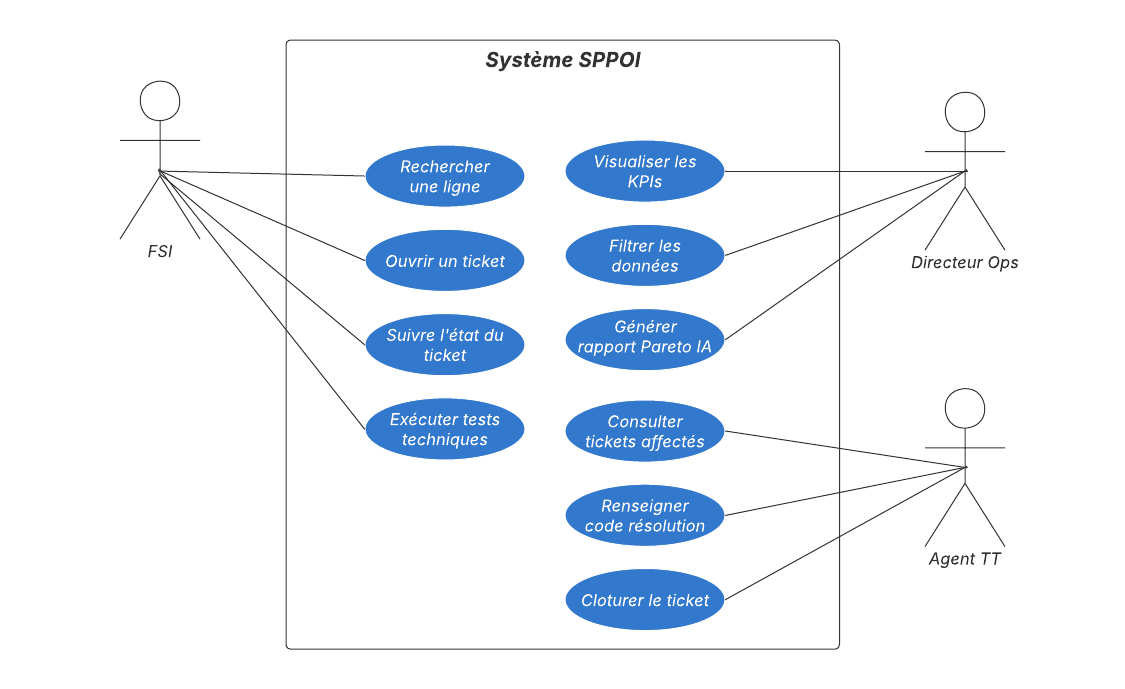
\includegraphics[width=0.9\textwidth]{imgs/diagramme-cas-utilisation.png}
\caption{Diagramme de cas d'utilisation --- Système SPPOI}
\label{fig:usecase}
\end{figure}

\subsection{Diagramme de classes}

Le diagramme de classes du système est organisé en quatre blocs fonctionnels qui reflètent l'architecture modulaire du SPPOI~:

\begin{itemize}[leftmargin=*, itemsep=4pt]
  \item \textbf{Bloc 1 -- Modèles de données~:} définit les entités Prisma \texttt{Client} (attributs~: DLigne, référence HPSM, statut, code résolution, région, offre), \texttt{Technicien} (employeeId, nom, email) et \texttt{Intervention} (productType, resolutionCode, status). Les relations~: un Client peut avoir plusieurs Interventions~; un Technicien effectue plusieurs Interventions.
  \item \textbf{Bloc 2 -- Services métier~:} regroupe les services d'authentification (NextAuth avec CredentialsProvider), la synchronisation des données depuis le fichier Excel (WorkbookSync), et les utilitaires de gestion des sessions.
  \item \textbf{Bloc 3 -- API Routes et contrôleurs~:} expose les endpoints REST pour les opérations CRUD (clients, interventions, synchronisation), le dashboard (KPIs, filtrage), et le module Pareto intelligent (génération de rapport IA via Groq).
  \item \textbf{Bloc 4 -- Utilitaires et modules~:} inclut le moteur de métriques (calcul des KPIs, Pareto, tendances), le module AI (construction de prompts, appel Groq/Llama~3.3~70B), et les vérifications d'environnement (runtime, fallback workbook).
\end{itemize}

\begin{figure}[H]
\centering
\begin{subfigure}[b]{0.48\textwidth}
\centering
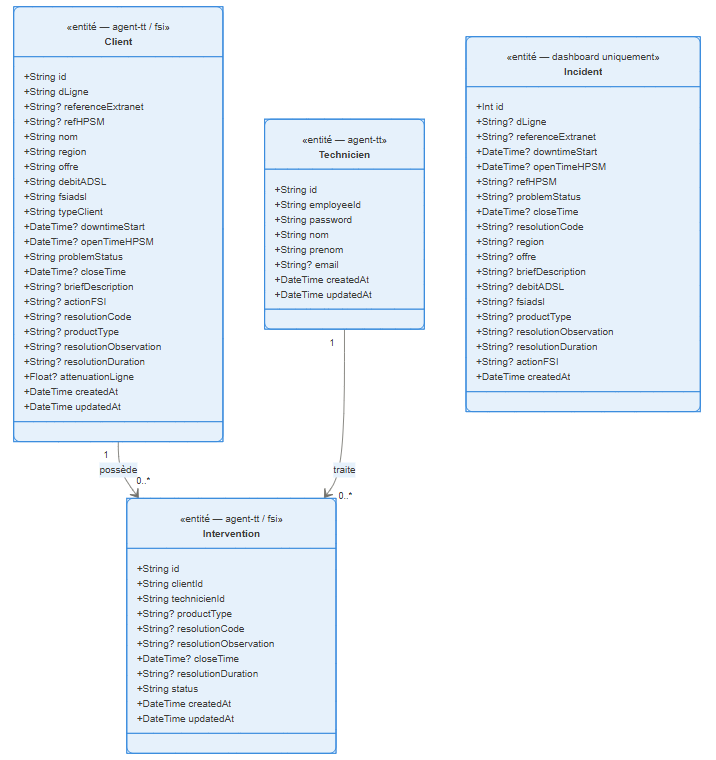
\includegraphics[width=\textwidth]{imgs/bloc1.png}
\caption{Modèles de données (Client, Technicien, Intervention)}
\label{fig:classes-bloc1}
\end{subfigure}
\hfill
\begin{subfigure}[b]{0.48\textwidth}
\centering
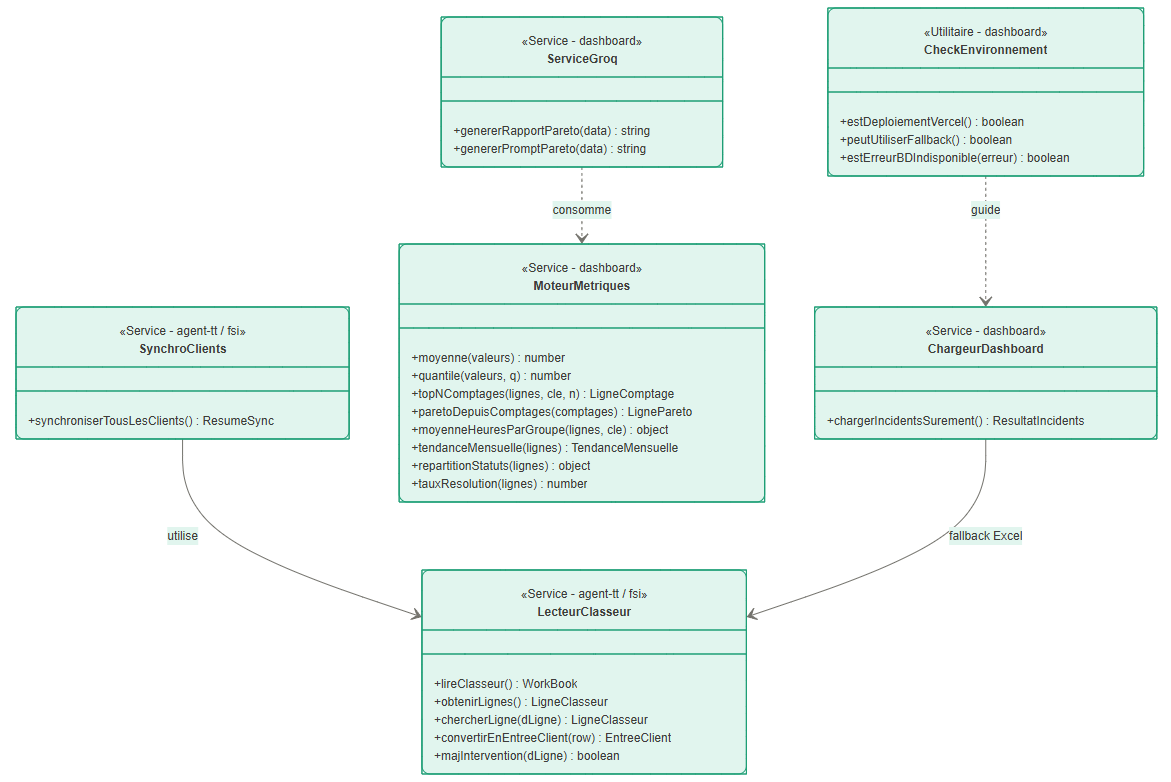
\includegraphics[width=\textwidth]{imgs/bloc2.png}
\caption{Services métier (Auth, Sync, Workbook)}
\label{fig:classes-bloc2}
\end{subfigure}

\bigskip

\begin{subfigure}[b]{0.48\textwidth}
\centering
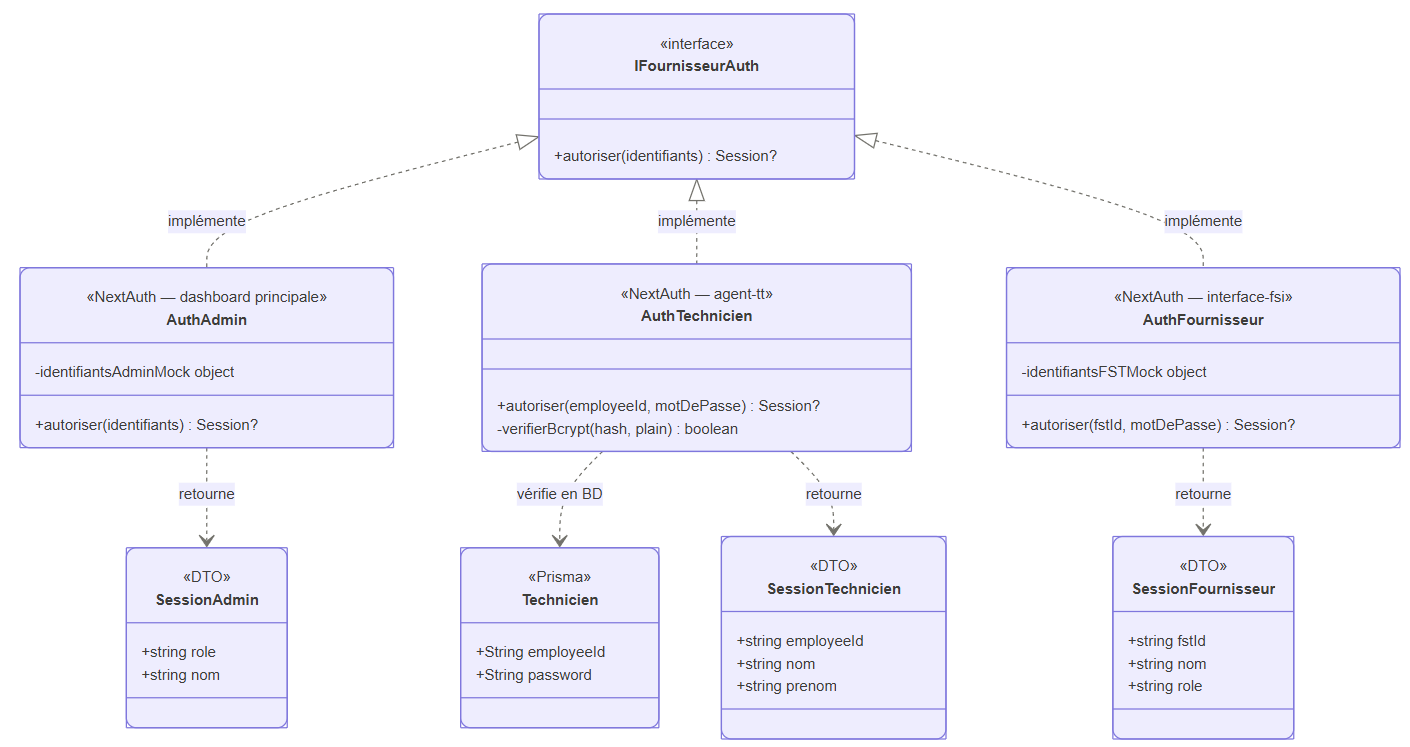
\includegraphics[width=\textwidth]{imgs/bloc3.png}
\caption{API Routes et contrôleurs}
\label{fig:classes-bloc3}
\end{subfigure}
\hfill
\begin{subfigure}[b]{0.48\textwidth}
\centering
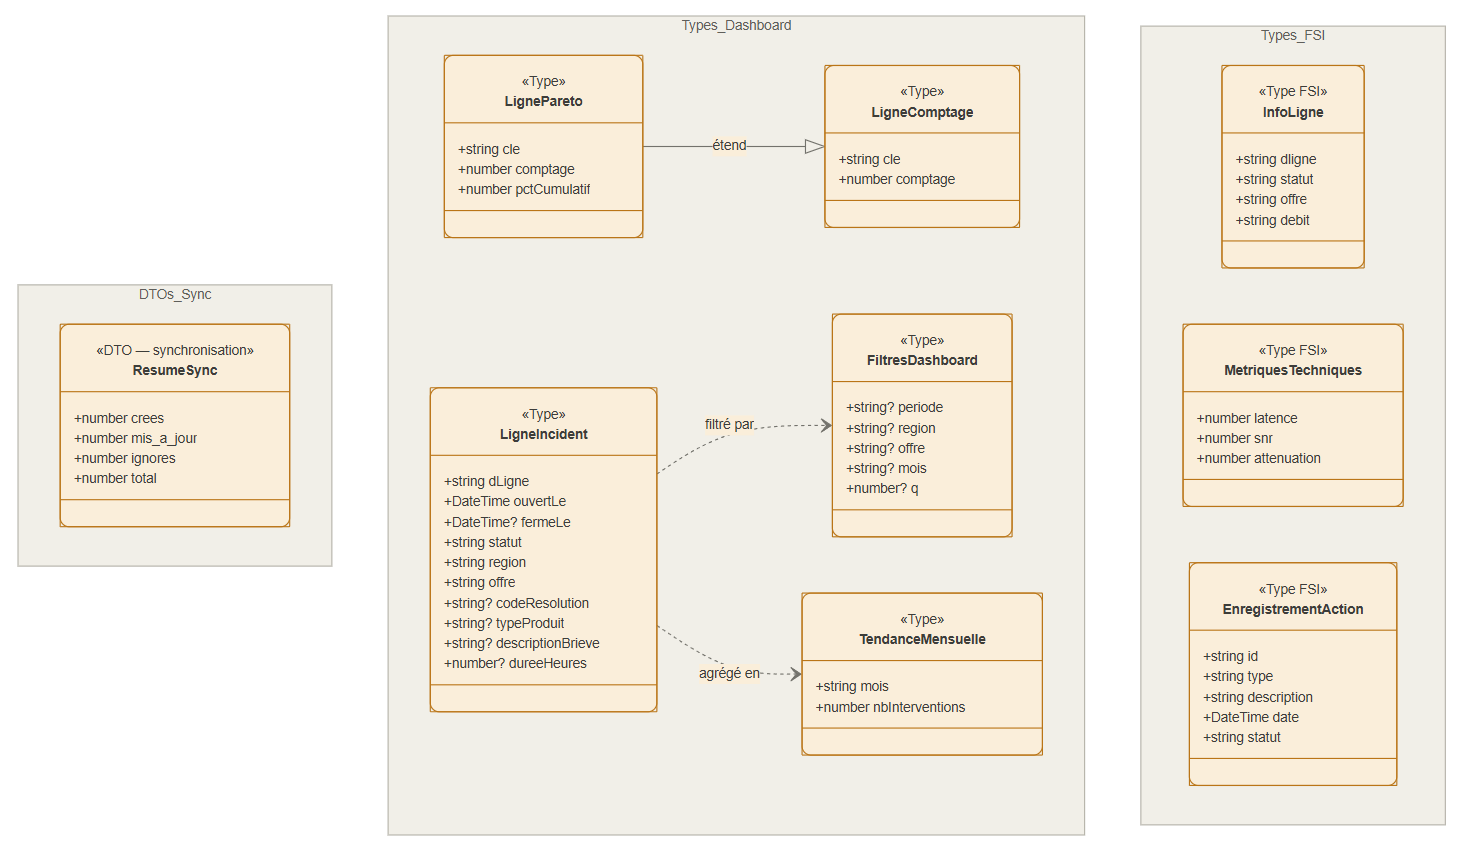
\includegraphics[width=\textwidth]{imgs/bloc4.png}
\caption{Utilitaires et modules (Metrics, AI, Runtime)}
\label{fig:classes-bloc4}
\end{subfigure}
\caption{Diagramme de classes --- Entités du système SPPOI (4 blocs)}
\label{fig:classes}
\end{figure}

\subsection{Diagrammes de séquence}

Deux diagrammes de séquence principaux ont été modélisés pour décrire les flux d'interaction les plus critiques du système.

\textbf{Séquence 1 --- Ouverture et suivi d'un ticket~:} Le FSI saisit le numéro de ligne dans l'Espace Fournisseur. Le système vérifie si un ticket est déjà ouvert pour cette ligne (contrôle de doublon). Si c'est un premier ticket, le FSI renseigne les détails de l'incident~; sinon, il consulte l'état du ticket existant. Après validation, le ticket est enregistré dans le système HPSM et apparaît dans l'Interface Agent TT.

\textbf{Séquence 2 --- Génération du rapport Pareto IA~:} Le Directeur des Opérations clique sur « Générer le rapport » dans la vue Pareto. Le système agrège les données filtrées, calcule le tableau Pareto, construit le prompt et appelle l'API Groq. Le modèle Llama\,3.3\,70B traite le prompt et retourne le rapport en langage naturel, qui est affiché dans l'interface en moins de 10\,secondes.

\subsection{Diagramme d'activité}

Le diagramme d'activité modélise le flux de traitement complet d'une réclamation, depuis le signalement du client jusqu'à la clôture du ticket et l'alimentation du dashboard. Le flux principal débute par le \textbf{Client} qui contacte l'\textbf{Espace Fournisseur} pour signaler un dérangement. Le FSI procède à la \textbf{recherche du numéro de ligne} (Search Number), ce qui déclenche une vérification de l'historique~:

\begin{itemize}[leftmargin=*, itemsep=4pt]
  \item \textbf{Première réclamation (First Time)~:} le FSI renseigne les détails de l'incident via le formulaire \textit{Add Details}, puis le ticket passe au statut \textbf{Cloturé} après validation initiale.
  \item \textbf{Réclamation existante (Not First Time)~:} le système vérifie l'état du ticket existant via \textit{Check Status}. Si le ticket est déjà clôturé, les tests techniques (\textit{Execute Tests}) sont exécutés~; si le ticket est en cours de traitement (\textit{Ouvert / Traitement}), il est routé vers l'\textbf{Interface Agent TT}.
\end{itemize}

Les \textbf{tests techniques} produisent deux issues~: \textbf{Pass} (tests concluants) renvoie au statut \textbf{Cloturé}, tandis que \textbf{Fail} (échec des tests) redirige vers \textit{Ouvert / Traitement} et l'Interface Agent TT pour une intervention corrective. Une \textbf{réparation/intervention} peut également être initiée directement depuis l'Interface Agent TT.

L'\textbf{Interface Agent TT} alimente la \textbf{base de données} avec les résultats d'intervention (code de résolution, durée, statut). La base de données synchronise les statuts \textbf{Cloturé} et \textbf{Ouvert/Traitement} en temps réel. Enfin, les données consolidées sont exploitées par le \textbf{Dashboard Principale} pour la visualisation des KPIs, alimentant le module \textbf{AI Agent} qui génère les rapports \textbf{Pareto Analysis} intelligents.

\begin{figure}[H]
\centering
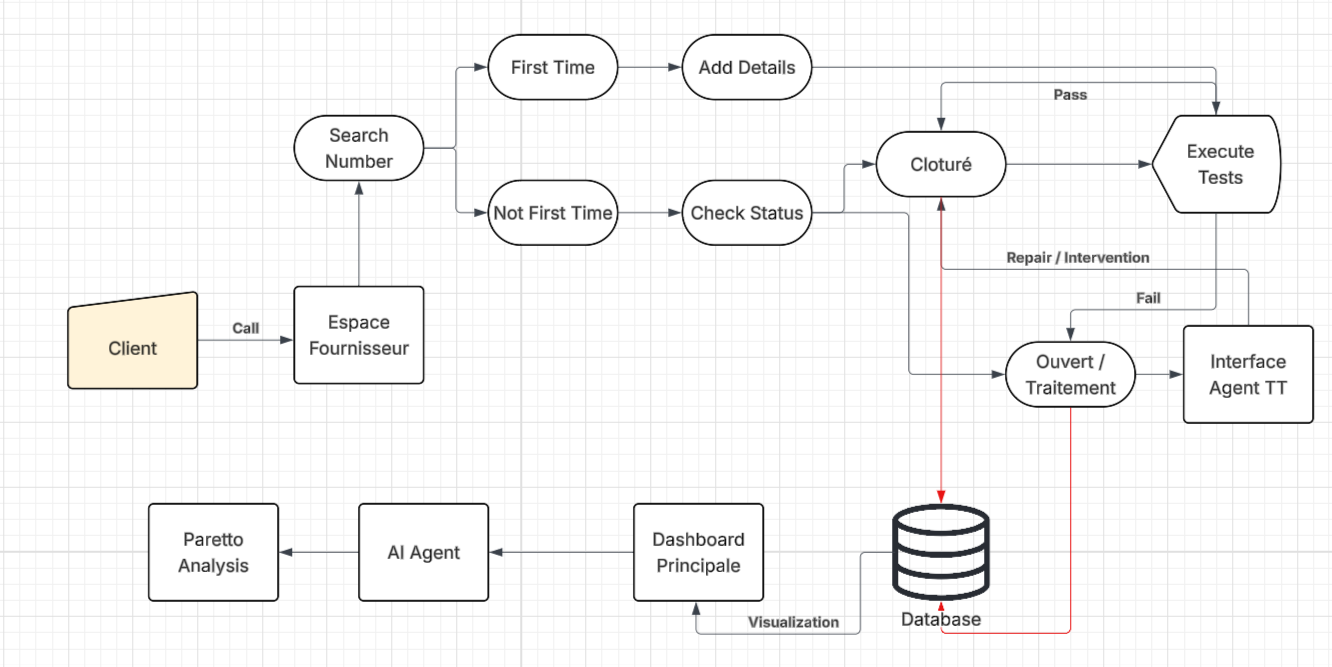
\includegraphics[width=0.95\textwidth]{../architecture.png}
\caption{Diagramme d'activité --- du signalement à la clôture du ticket}
\label{fig:activity}
\end{figure}

\section{Architecture Applicative Globale}

\subsection{Architecture en couches du système}

Le système est articulé autour d'une architecture applicative en \textbf{trois couches} distinctes~:

\begin{table}[H]
\centering
\caption{Architecture en couches du système SPPOI}
\begin{tabularx}{\textwidth}{L{3.5cm} L{3cm} X}
\toprule
\rowcolor{ttlblue}
\textbf{\color{ttblue}Couche} & \textbf{\color{ttblue}Technologie} & \textbf{\color{ttblue}Composants} \\
\midrule
Présentation (UI) & Next.js (App Router) + Tailwind CSS + Recharts & Espace FSI, Interface Agent TT, Dashboard Principale (10 vues) \\
\rowcolor{ttlgray}
Métier (serveur) & Route Handlers Next.js + Zod + Groq API & Validation des requêtes, filtrage multicritère, agrégation Pareto, génération de rapport IA \\
Données & Prisma ORM + source Excel SheetJS & Persistance métier (\texttt{Client}, \texttt{Intervention}, \texttt{Technicien}, \texttt{Incident}), synchronisation et repli analytique \\
\bottomrule
\end{tabularx}
\label{tab:archi-couches}
\end{table}

\section{Conception des Indicateurs de Performance}

\subsection{Cartographie des KPIs retenus}

Sur la base du diagnostic et des besoins exprimés par la Direction des Opérations, cinq indicateurs clés de performance ont été retenus, formalisés et intégrés dans le dashboard~:

\begin{table}[H]
\centering
\caption{Cartographie complète des KPIs retenus et leurs paramètres de pilotage}
\begin{tabularx}{\textwidth}{L{3.2cm} L{3.5cm} L{3cm} L{2.5cm}}
\toprule
\rowcolor{ttlblue}
\textbf{\color{ttblue}KPI} & \textbf{\color{ttblue}Définition} & \textbf{\color{ttblue}Formule de calcul} & \textbf{\color{ttblue}Valeur cible} \\
\midrule
Total Incidents & Volume total de réclamations dans le périmètre filtré & COUNT(tickets) & Suivi continu \\
\rowcolor{ttlgray}
Taux de Résolution & Part des tickets clôturés sur le total & $\frac{\text{Clôturés}}{\text{Total}} \times 100$ & $\geq$ 99,5\,\% \\
Délai Moyen & Durée moyenne de traitement en heures & AVG(TT\_resolution\_duration) & $\leq$ 72\,h (SLA) \\
\rowcolor{ttlgray}
Tickets Urgents & Tickets avec délai $>$ 72\,h (SLA breach) & COUNT(durée $>$ 72h) & $<$ 5\,\% du total \\
Délai Maximum & Délai maximum observé sur la période & MAX(TT\_resolution\_duration) & Alerte si $>$ 240\,h \\
\bottomrule
\end{tabularx}
\label{tab:kpis-conception}
\end{table}

\subsection{Définition des seuils et alertes automatiques}

Chaque KPI est associé à un système d'alertes visuelles à trois niveaux~: \textcolor{ttgreen}{\textbf{vert}} (performance conforme à la cible), \textcolor{ttorange}{\textbf{orange}} (dérive détectée --- attention requise) et \textcolor{ttred}{\textbf{rouge}} (seuil critique dépassé --- action corrective urgente). Sur les données réelles analysées, \textbf{23,1\,\% des tickets} (5\,278 tickets) déclenchent l'alerte critique rouge, justifiant pleinement la mise en place d'un système de monitoring automatisé.

\section{Conception de la Base de Données}

\subsection{Structure du fichier de données source (\texttt{all-data.xlsx})}

Le fichier \texttt{all-data.xlsx} fourni par le Fournisseur Anonyme constitue la \textbf{source de données de référence} utilisée pour l'import, la synchronisation et les traitements analytiques. Ce classeur regroupe l'ensemble des tickets de réclamation traités sur l'année 2025~: \textbf{22\,851 enregistrements}, couvrant la période du 1\textsuperscript{er}~janvier 2025 au 30~décembre 2025, répartis en 17 champs. En parallèle, les applications métier s'appuient sur des modèles \textbf{Prisma} (\texttt{Client}, \texttt{Intervention}, \texttt{Technicien}) pour persister les actions FSI et les clôtures techniques réalisées dans les interfaces opérationnelles.

\subsection{Dictionnaire des données}

\begin{longtable}{L{4cm} L{2.5cm} L{7cm}}
\caption{Dictionnaire des données --- Fichier all-data.xlsx (Fournisseur Anonyme 2025)} \label{tab:dict} \\
\toprule
\rowcolor{ttlblue}
\textbf{\color{ttblue}Champ} & \textbf{\color{ttblue}Type} & \textbf{\color{ttblue}Description} \\
\midrule
\endfirsthead
\toprule
\rowcolor{ttlblue}
\textbf{\color{ttblue}Champ (suite)} & \textbf{\color{ttblue}Type} & \textbf{\color{ttblue}Description} \\
\midrule
\endhead
\bottomrule
\endfoot
DLigne                      & Texte      & Identifiant unique de la ligne cliente \\
\rowcolor{ttlgray}
reference\_no Extranet      & Texte      & Référence du ticket sur le portail Extranet FSI \\
downtime\_start (Extranet)  & Date/Heure & Date et heure de début de l'incident signalé par le FSI \\
\rowcolor{ttlgray}
open\_time (HPSM)           & Date/Heure & Date et heure d'ouverture du ticket dans le système HPSM \\
Ref HPSM                    & Texte      & Référence unique du ticket dans le système HPSM \\
\rowcolor{ttlgray}
problem\_status             & Texte      & Statut du ticket~: Clôturé (99,9\,\%) ou Ouvert (0,1\,\%) \\
close\_time                 & Date/Heure & Date et heure de clôture du ticket \\
\rowcolor{ttlgray}
resolution\_code            & Texte      & Code de résolution de l'intervention TT (PC, Aucun, IPMSAN, etc.) \\
Region                      & Texte      & Région géographique de la ligne cliente (24 régions distinctes) \\
\rowcolor{ttlgray}
Offre                       & Texte      & Offre commerciale souscrite (ADSL Hybride, VDSL, etc.) \\
brief\_description          & Texte      & Description courte du motif de réclamation (pas de synchro, etc.) \\
\rowcolor{ttlgray}
product\_type               & Texte      & Famille d'intervention TT (Rien à signaler, Fixation Coffret, etc.) \\
TT\_resolution\_duration    & Durée      & Durée totale de traitement du ticket au format JJ\,HH:MM:SS \\
\end{longtable}

\section{Conception des Interfaces Utilisateur (Maquettes)}

\subsection{Maquette de l'espace fournisseur FSI}

L'interface Fournisseur (Espace FSI) est structurée autour d'un \textbf{écran de connexion}, puis d'un \textbf{dashboard opérateur} centré sur la recherche par \texttt{DLigne}. Après recherche, le fournisseur visualise les détails de la ligne, peut lancer une \textbf{synchronisation explicite Excel $\rightarrow$ base}, puis renseigne un \textbf{formulaire guidé multi-étapes} pour tracer l'action FSI. Si aucune ligne n'existe encore, l'interface propose un scénario \textbf{Ajouter nouveau} permettant de créer le premier ticket avec les champs métier obligatoires (date de panne, région, offre, débit, FSI, description). Le résultat des tests est enregistré en base avec un statut métier orienté vers le traitement côté Tunisie Telecom.

\begin{figure}[H]
\centering
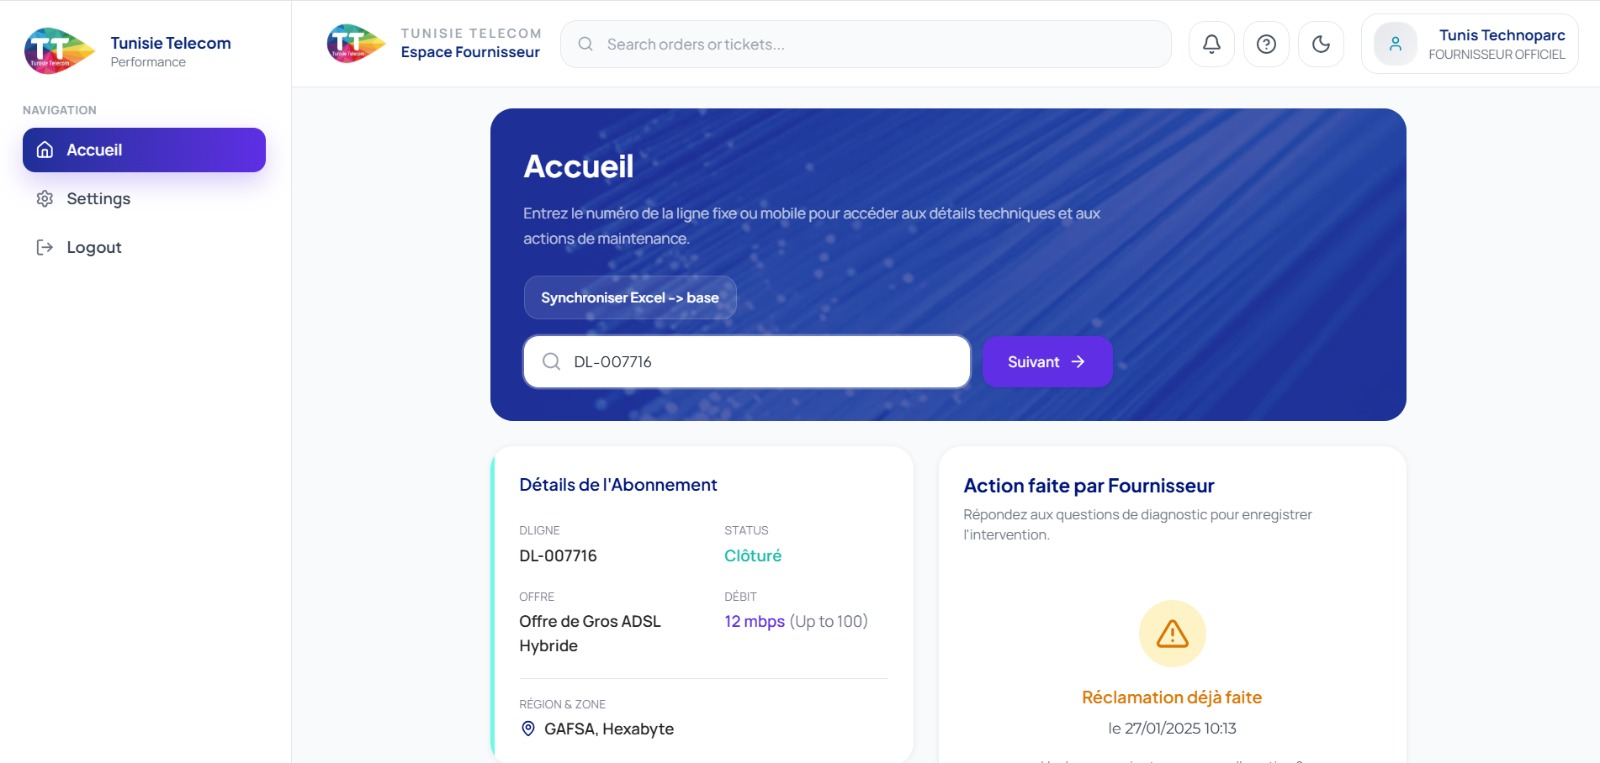
\includegraphics[width=0.85\textwidth]{imgs/01-fsi-interface.jpeg}
\caption{Interface Fournisseur FSI --- Ouverture et suivi de ticket}
\label{fig:fsi}
\end{figure}

\subsection{Maquette de l'interface agent technicien TT}

L'Interface Agent TT présente une vue d'accueil orientée recherche, une liste des interventions en cours/terminées, ainsi qu'un écran de détail permettant au technicien de renseigner le code de résolution, la famille d'intervention (\texttt{product\_type}) et ses observations terrain. La validation d'une intervention crée un enregistrement \texttt{Intervention}, met à jour le client associé dans \texttt{Prisma}, calcule la \texttt{resolution\_duration} et positionne le ticket au statut \textbf{Clôturé}. En environnement local compatible, la clôture peut également répercuter ces valeurs dans le classeur Excel de travail.

\begin{figure}[H]
\centering
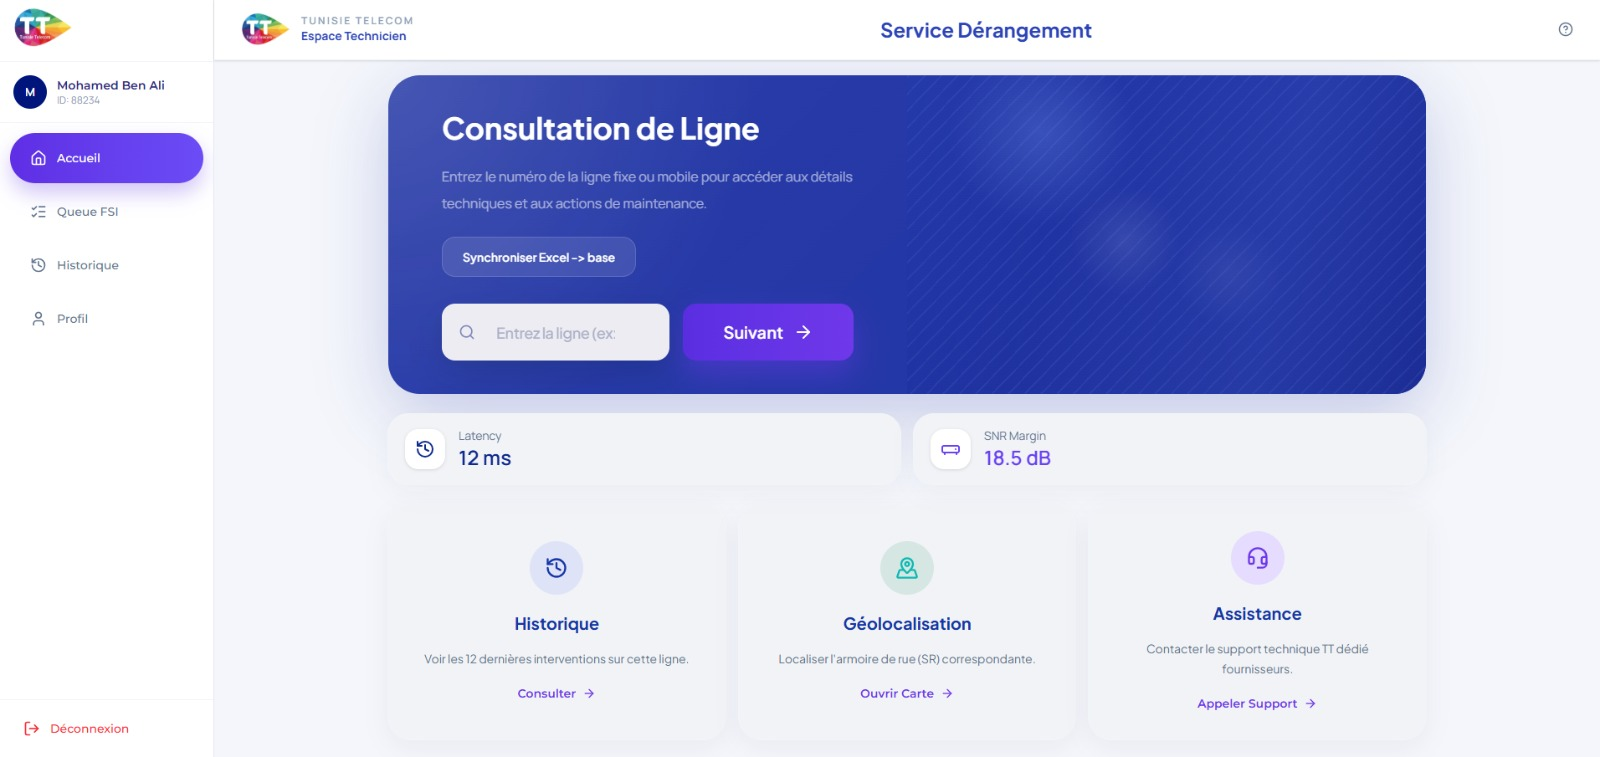
\includegraphics[width=0.85\textwidth]{imgs/02-agent-tt.jpeg}
\caption{Interface Agent TT --- Consultation et clôture des interventions}
\label{fig:agent-tt}
\end{figure}

\subsection{Maquette du dashboard de performance principale}

Le Dashboard Principale est organisé en une navigation latérale (sidebar) donnant accès à dix vues analytiques~: Vue Globale, Réclamations, Interventions, Performance, Offres \& Produits, Pareto, et les opérations détaillées (Régions, Résolutions TT, Actions FSI, Détail Lignes). Les filtres transverses sont portés par l'URL (\texttt{period}, \texttt{region}, \texttt{offer}, \texttt{month}, \texttt{q}), ce qui garantit à la fois la synchronisation des vues et la partageabilité des analyses.

\begin{figure}[H]
\centering
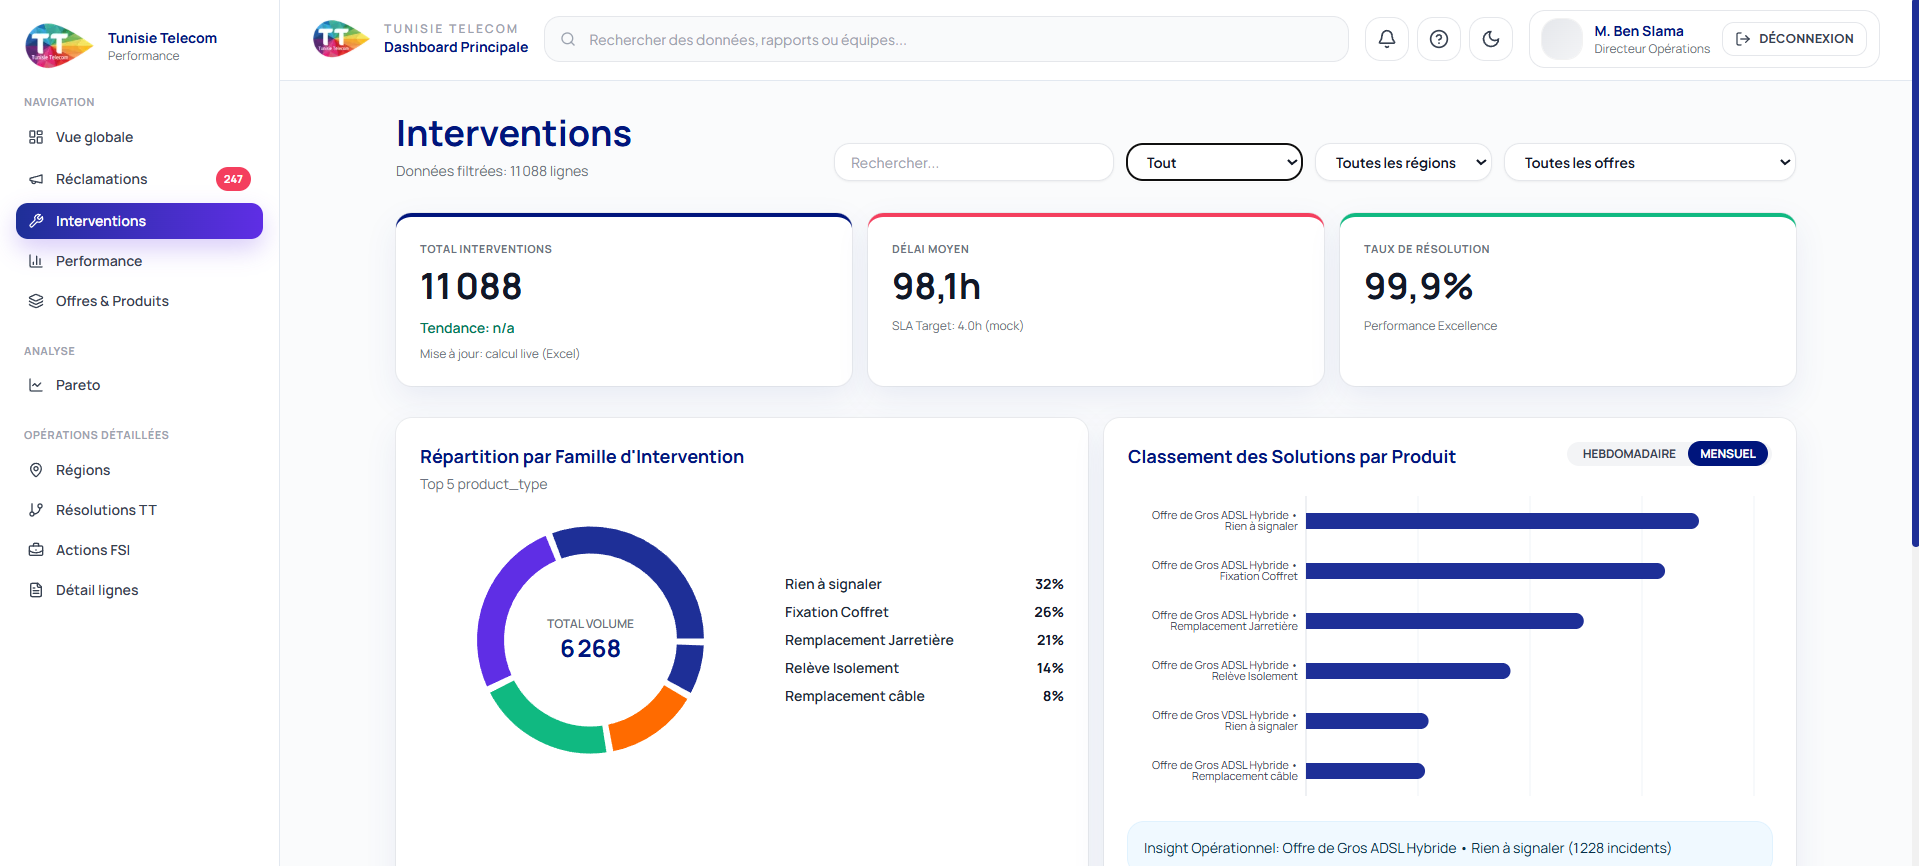
\includegraphics[width=0.85\textwidth]{imgs/03-dashboard-interventions.png}
\caption{Dashboard Principale --- Capture d'un tableau de bord opérationnel}
\label{fig:dashboard-global}
\end{figure}

\chapconclusion{%
Cette phase de conception a permis de structurer précisément les composants du système, leurs responsabilités et leurs interactions. L'architecture obtenue fournit un cadre solide pour une implémentation modulaire, décrite dans le chapitre suivant à travers les choix techniques et les réalisations concrètes.%
}


% ═════════════════════════════════════════════════════════════════════════════
%  CHAPITRE 4
% ═════════════════════════════════════════════════════════════════════════════
\chapter{Réalisation et Implémentation}

\chapintro{%
Ce chapitre présente la matérialisation technique du système conçu. Il détaille l'implémentation du dashboard analytique, du module Pareto intelligent et des interfaces métier, en mettant l'accent sur les technologies employées et sur la cohérence entre conception et réalisation.%
}


\section{Environnement de Développement}

\subsection{Stack technique utilisé}

Le système de pilotage de la performance organisationnelle a été développé en s'appuyant sur un ensemble de technologies modernes, sélectionnées pour leur performance, leur maintenabilité et leur adéquation avec les besoins fonctionnels~:

\begin{table}[H]
\centering
\caption{Stack technique complet du système SPPOI}
\begin{tabularx}{\textwidth}{L{3cm} L{4.5cm} X}
\toprule
\rowcolor{ttlblue}
\textbf{\color{ttblue}Composant} & \textbf{\color{ttblue}Technologie} & \textbf{\color{ttblue}Rôle dans le système} \\
\midrule
Framework Web  & Next.js (App Router)    & Développement fullstack, rendu serveur et Route Handlers backend \\
\rowcolor{ttlgray}
Langage        & TypeScript / JavaScript & Typage statique et développement applicatif robuste \\
Visualisation  & Recharts                & Graphiques KPI, Pareto, tendances, camemberts, barres \\
\rowcolor{ttlgray}
IA / LLM       & Groq API + Llama\,3.3\,70B & Génération des rapports Pareto intelligents en FR \\
Base de données & Prisma + classeur Excel & Persistance métier, synchronisation des données et repli analytique \\
\rowcolor{ttlgray}
Style          & Tailwind CSS            & Design system utility-first et responsive layout \\
Déploiement    & Vercel                  & Hébergement cloud CDN mondial et CI/CD automatisé \\
\rowcolor{ttlgray}
Versioning     & Git / GitHub            & Gestion du code source et collaboration \\
\bottomrule
\end{tabularx}
\label{tab:stack}
\end{table}

\section{Analyse Exploratoire des Données (EDA)}

\subsection{Description et qualité du jeu de données}

Le fichier \texttt{all-data.xlsx} fourni par le Fournisseur Anonyme constitue la source de données primaire du volet analytique. Il contient \textbf{22\,851 enregistrements} de réclamations et interventions couvrant l'intégralité de l'année 2025 (du 1\textsuperscript{er}~janvier au 30~décembre), répartis sur \textbf{24 régions géographiques}, \textbf{24 offres commerciales} distinctes et \textbf{12 codes de résolution}. Cette source est relue côté serveur soit directement depuis le classeur, soit via la table \texttt{Incident} importée dans Prisma lorsqu'une base est configurée, ce qui permet de conserver la même logique de calcul indépendamment du runtime.

\subsection{Distribution des délais de résolution}

L'analyse statistique de la durée de résolution des tickets révèle une distribution fortement asymétrique à droite, caractéristique des processus de maintenance~:

\begin{table}[H]
\centering
\caption{Statistiques descriptives du délai de résolution --- Fournisseur Anonyme 2025}
\begin{tabularx}{\textwidth}{L{4cm} C{3cm} L{7cm}}
\toprule
\rowcolor{ttlblue}
\textbf{\color{ttblue}Statistique} & \textbf{\color{ttblue}Valeur} & \textbf{\color{ttblue}Interprétation} \\
\midrule
Délai minimum         & 0,0\,h    & Résolution immédiate (diagnostic à distance réussi) \\
\rowcolor{ttlgray}
Médiane               & 25,8\,h   & 50\,\% des tickets résolus en moins d'un jour \\
Délai moyen           & 79,0\,h   & Tiré vers le haut par les incidents complexes \\
\rowcolor{ttlgray}
Tickets $\leq$ 24\,h  & 10\,366 (45,4\,\%) & Quasi-moitié des tickets résolus en moins d'un jour \\
Tickets $>$ 72\,h     & 5\,278 (23,1\,\%) & Tickets urgents (SLA breach) à traiter en priorité \\
\rowcolor{ttlgray}
Délai maximum         & 4\,344,4\,h & Soit 181\,jours --- incident infrastructurel exceptionnel \\
\bottomrule
\end{tabularx}
\label{tab:stats-delai}
\end{table}

\insight{Paradoxe Performance/Délais}{Le taux de résolution excellent de 99,93\,\% coexiste avec un délai moyen élevé (79,0\,h). Ce paradoxe s'explique par la coexistence de deux populations~: 45,4\,\% des tickets résolus en moins de 24\,h (incidents courants à résolution rapide) et 23,1\,\% de tickets urgents dépassant 72\,h (incidents infrastructurels complexes). La médiane (25,8\,h) reflète mieux la performance typique que la moyenne (79,0\,h), qui est tirée vers le haut par quelques incidents exceptionnels à durée très longue.}

\subsection{Analyse des volumes par région, offre et famille}

L'analyse des volumes révèle les concentrations suivantes~:

\begin{itemize}[leftmargin=*, itemsep=4pt]
  \item \textbf{Par région~:} GAFSA concentre le volume le plus élevé (4\,560 tickets --- 20,0\,\%), suivi de TUNIS (2\,043 --- 8,9\%), BÉJA (1\,647 --- 7,2\%) et KASSERINE (1\,502 --- 6,6\%).
  \item \textbf{Par offre~:} L'Offre de Gros ADSL Hybride domine largement avec 15\,163 tickets (66,4\,\%), reflétant la base installée ADSL prépondérante dans le réseau du Fournisseur Anonyme.
  \item \textbf{Par famille d'intervention~:} « Rien à signaler » représente 20,3\,\% (4\,570 tickets), signifiant qu'un ticket sur cinq n'aboutit à aucune action corrective côté TT --- signal d'alerte important sur la qualité du diagnostic préalable du FSI.
\end{itemize}

\subsection{Saisonnalité des incidents et corrélations}

L'analyse de la distribution mensuelle des tickets révèle une saisonnalité marquée~:

\begin{table}[H]
\centering
\caption{Distribution mensuelle des tickets --- Fournisseur Anonyme 2025}
\begin{tabularx}{\textwidth}{C{1.5cm} C{2.5cm} C{2.5cm} C{2.5cm} C{2.5cm} C{2.5cm}}
\toprule
\rowcolor{ttlblue}
\textbf{\color{ttblue}Mois} & \textbf{\color{ttblue}Jan.} & \textbf{\color{ttblue}Fév.} & \textbf{\color{ttblue}Mar.} & \textbf{\color{ttblue}Avr.} & \textbf{\color{ttblue}Mai} \\
\midrule
Volume & 1\,994 & 1\,708 & 1\,708 & 1\,941 & 2\,054 \\
\rowcolor{ttlblue}
\textbf{\color{ttblue}Mois} & \textbf{\color{ttblue}Juin} & \textbf{\color{ttblue}Juil.} & \textbf{\color{ttblue}Août} & \textbf{\color{ttblue}Sep.} & \textbf{\color{ttblue}Oct--Déc.} \\
\rowcolor{white}
Volume & 1\,974 & \textbf{2\,129} & 1\,864 & 1\,946 & 1\,533 (moy.) \\
\bottomrule
\end{tabularx}
\label{tab:monthly}
\end{table}

Le pic de juillet~2025 (2\,129 tickets --- volume mensuel maximum) s'explique par les effets thermiques sur l'infrastructure réseau cuivre (dilatation des câbles, dégradation des connecteurs) lors des périodes de forte chaleur estivale. Les mois de février et mars~2025 affichent les volumes les plus faibles (1\,708 tickets chacun), correspondant à une période de faible activité thermique et de moindre sollicitation du réseau.

\section{Traitement des Données et Calcul des KPIs}

\subsection{Chargement et parsing du fichier source (SheetJS)}

Les données analytiques sont chargées côté serveur via une stratégie à deux niveaux~: lecture prioritaire depuis \textbf{Prisma} lorsqu'une base est configurée, sinon repli vers le fichier \texttt{all-data.xlsx} via \textbf{SheetJS}. Chaque enregistrement normalisé est enrichi de champs calculés~:

\begin{itemize}[leftmargin=*, itemsep=4pt]
  \item \textbf{Délai de résolution en heures~:} converti depuis le format natif JJ\,HH:MM:SS du champ \texttt{TT\_resolution\_duration} via une fonction de parsing dédiée.
  \item \textbf{Mois d'ouverture~:} extrait du champ \texttt{open\_time (HPSM)} pour les analyses de tendance mensuelle.
  \item \textbf{Cluster d'offre~:} regroupement de l'offre commerciale en trois catégories (ADSL, VDSL, AUTRES/DATA) pour les analyses macro.
  \item \textbf{Statut d'urgence~:} booléen calculé automatiquement (délai $>$ 72\,h = ticket urgent = SLA breach).
\end{itemize}

\subsection{Calcul des indicateurs clés de performance}

Les cinq KPIs principaux du dashboard sont calculés dynamiquement lors du rendu serveur des pages analytiques, en appliquant les filtres sélectionnés par l'utilisateur. La logique de filtrage multicritère permet de combiner simultanément un filtre temporel (période), un filtre géographique (région) et un filtre commercial (offre), garantissant la cohérence des données à travers l'ensemble des dix vues du dashboard.

\subsection{Logique de filtrage multicritère}

Le système de filtres globaux persistants est implémenté via les \textbf{paramètres d'URL} partagés entre toutes les vues. Lorsqu'un filtre est modifié (ex.~: sélection de la région « Grand Tunis »), la page est recalculée avec les nouvelles valeurs \texttt{period}, \texttt{region}, \texttt{offer}, \texttt{month} et \texttt{q}, garantissant la cohérence des données affichées et la possibilité de partager un état d'analyse exact. Les filtres exposés dans l'interface sont~: période (30\,j, 90\,j, 365\,j, tout), région et offre commerciale, avec verrouillage mensuel optionnel sur certaines vues détaillées.

\section{Implémentation du Dashboard Principal}

\subsection{Architecture des composants React}

Le Dashboard Principale est structuré en un ensemble de composants React modulaires et réutilisables. La \textbf{sidebar} donne accès aux dix vues analytiques principales~; chaque vue est un composant Next.js autonome s'appuyant sur des bibliothèques partagées de normalisation, filtrage, métriques et formatage. Les composants graphiques (\texttt{KpiCards}, \texttt{ParetoComboChart}, \texttt{HorizontalBarChart}, \texttt{DonutChart}) sont réutilisables et paramétrables, tandis que la génération du rapport IA repose sur un \textit{Route Handler} dédié.

\subsection{Vue Globale --- Tableau de bord exécutif}

La Vue Globale constitue la page d'accueil du Dashboard Principale, conçue pour offrir au Directeur des Opérations une lecture synthétique et immédiate de l'état de la performance organisationnelle. Elle est structurée en trois niveaux de lecture~:

\begin{enumerate}[leftmargin=*, label=(\arabic*), itemsep=4pt]
  \item \textbf{KPI Cards de premier niveau~:} Total Incidents (11\,088 sur le périmètre filtré 30\,j), Taux de Résolution (99,9\,\%) et Délai Moyen (98,1\,h).
  \item \textbf{Graphiques analytiques~:} histogramme mensuel différenciant les flux Technique et Commercial~; donut chart des statuts globaux (Traités~: 11\,076, En cours~: 12, Urgents~: 2\,980).
  \item \textbf{Classements~:} Top Régions par volume (GAFSA, BÉJA, KASSERINE) et Top Offres par volume (ADSL Hybride en tête avec 7\,518 occurrences sur le périmètre filtré).
\end{enumerate}

\begin{figure}[H]
\centering
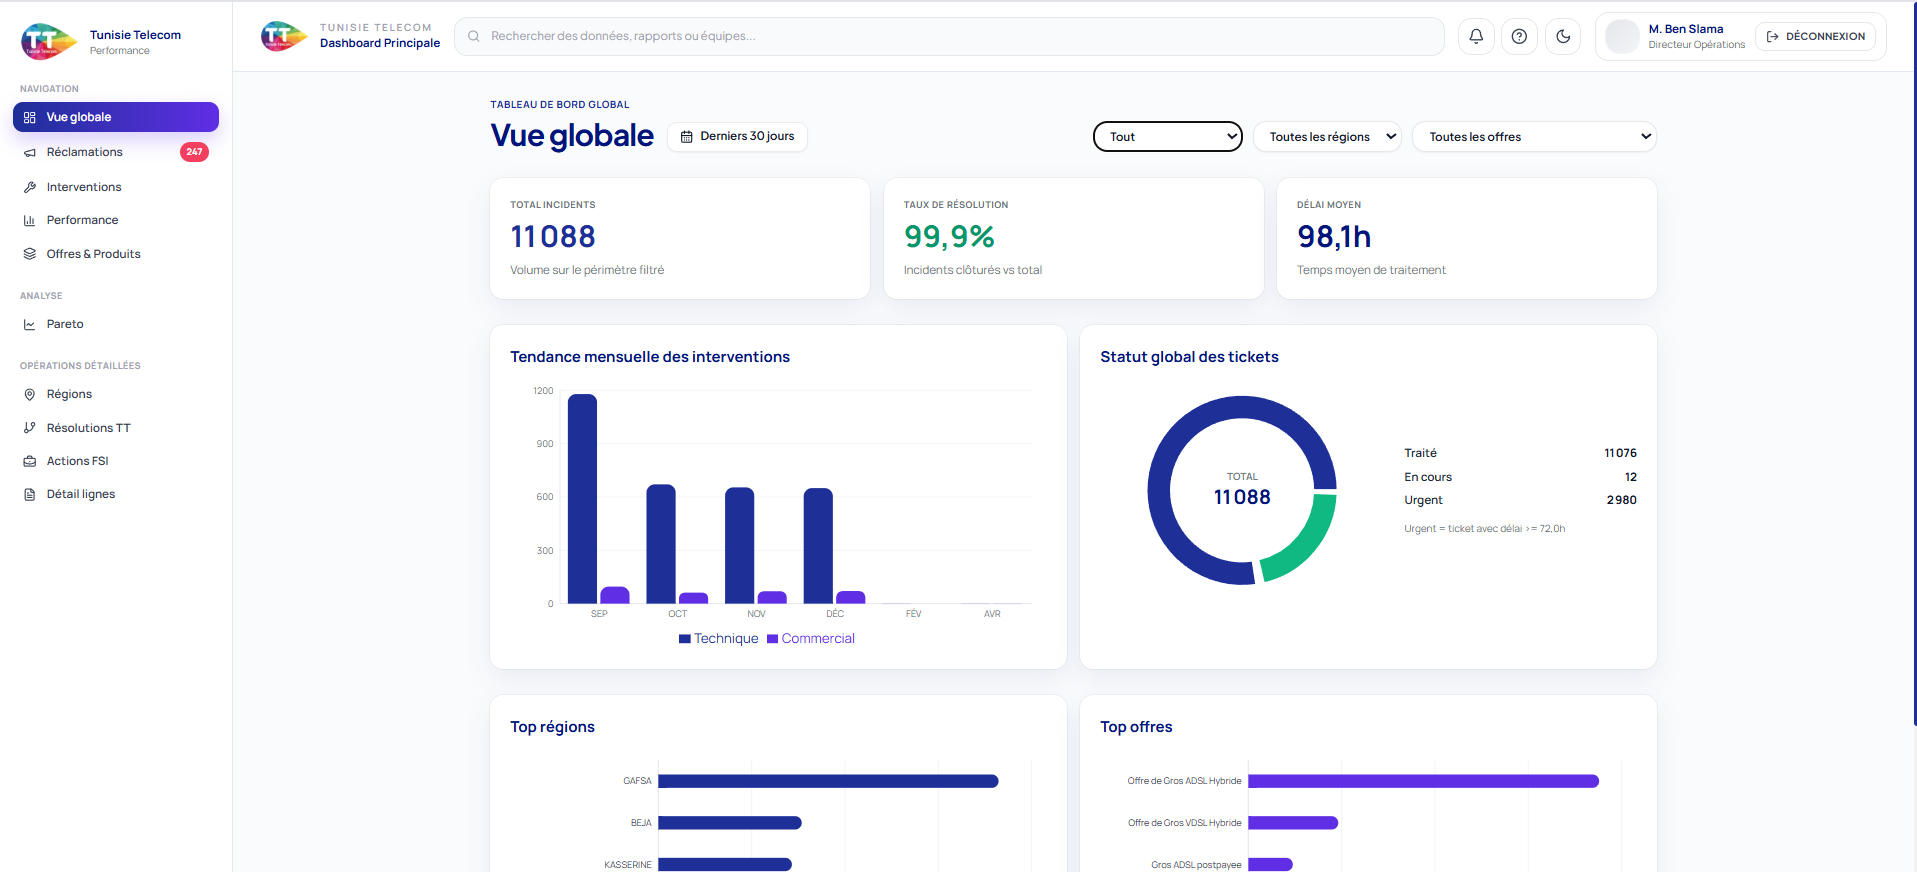
\includegraphics[width=0.85\textwidth]{imgs/00-dashboard-global.png}
\caption{Vue Globale --- Dashboard Principale --- Tableau de bord exécutif Tunisie Telecom}
\label{fig:vue-globale}
\end{figure}

\subsection{Vue Interventions --- Analyse des familles d'intervention}

La Vue Interventions présente l'analyse opérationnelle de la répartition des interventions par famille (\texttt{product\_type}) et par solution produit. Les résultats clés sur l'ensemble du dataset~:

\begin{itemize}[leftmargin=*, itemsep=4pt]
  \item \textbf{Rien à signaler~:} 4\,570 interventions (20,3\,\%) --- délai moyen de 21,2\,h (le plus bas de toutes les familles).
  \item \textbf{Fixation Coffret~:} 3\,364 interventions (14,7\,\%) --- délai moyen de 94,1\,h.
  \item \textbf{Remplacement Jarretière~:} 2\,608 interventions (11,4\,\%) --- délai moyen de 87,1\,h.
  \item \textbf{Relève Isolement~:} 1\,712 interventions (7,5\,\%) --- délai moyen de 85,2\,h.
  \item \textbf{Remplacement câble~:} 870 interventions (3,8\,\%) --- délai moyen de 146,4\,h (le plus élevé).
\end{itemize}

\begin{figure}[H]
\centering
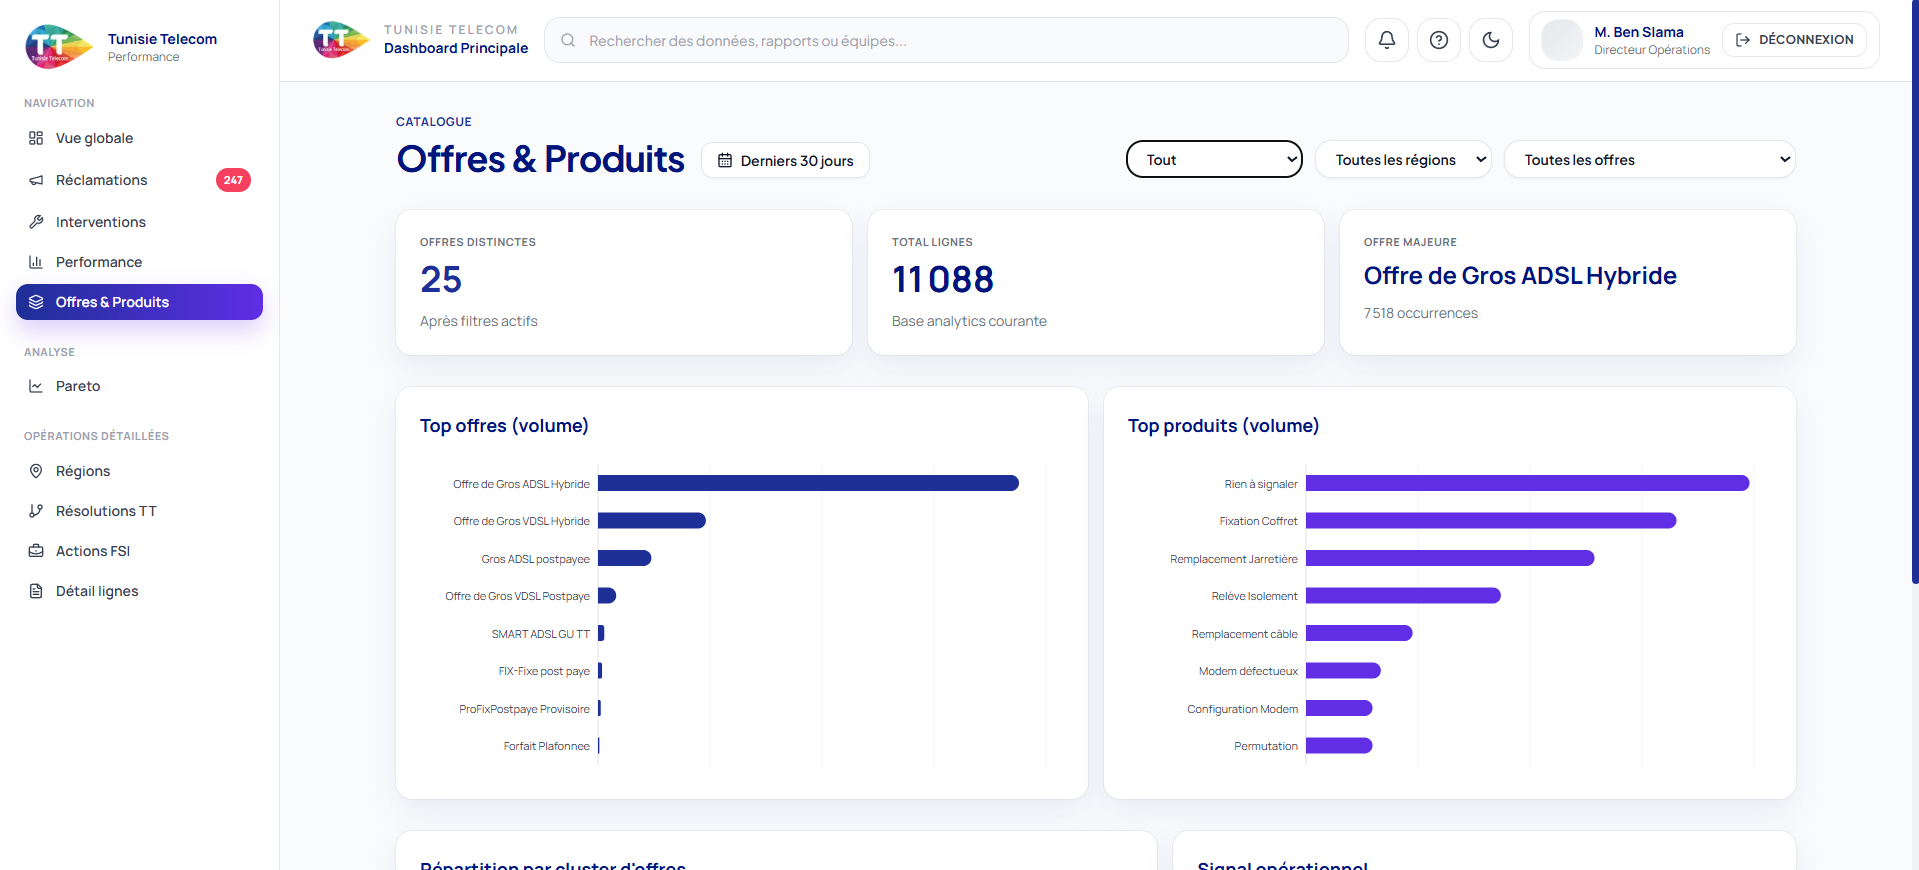
\includegraphics[width=0.85\textwidth]{imgs/05-dashboard-offres-produits.png}
\caption{Vue Offres \& Produits --- Catalogue et répartition des offres}
\label{fig:vue-interventions}
\end{figure}

\subsection{Vue Performance --- Analyse des délais}

La Vue Performance est dédiée à l'analyse multidimensionnelle des délais de résolution selon trois axes~:

\begin{enumerate}[leftmargin=*, label=(\arabic*), itemsep=6pt]
  \item \textbf{Délais par région géographique~:} Mannouba affiche le délai moyen le plus élevé (180,8\,h), suivi de Sousse (160,0\,h), Tataouine (145,8\,h) et Sidi Bouzid (145,2\,h). Ces disparités régionales importantes peuvent s'expliquer par des différences d'effectifs terrain, de densité du réseau ou de complexité des incidents locaux.

  \item \textbf{Délais par cluster d'offre~:} ADSL~: 82,6\,h (délai le plus élevé, reflétant l'âge du réseau cuivre et la complexité des incidents), VDSL~: 67,2\,h, Autres/Data~: 71,8\,h.

  \item \textbf{Délais par famille d'intervention TT~:} Technique Local~: 4,9\,j / 5\,042 interventions~; Technique Réseau~: 4,9\,j / 3\,120 interventions~; Service/Client~: 1,9\,j / 2\,926 interventions. La différence significative entre interventions techniques (4,9\,j) et service client (1,9\,j) s'explique par la nature des interventions~: les problèmes techniques nécessitent un déplacement terrain avec diagnostic physique, tandis que les interventions service client peuvent souvent être résolues à distance.
\end{enumerate}

\begin{figure}[H]
\centering
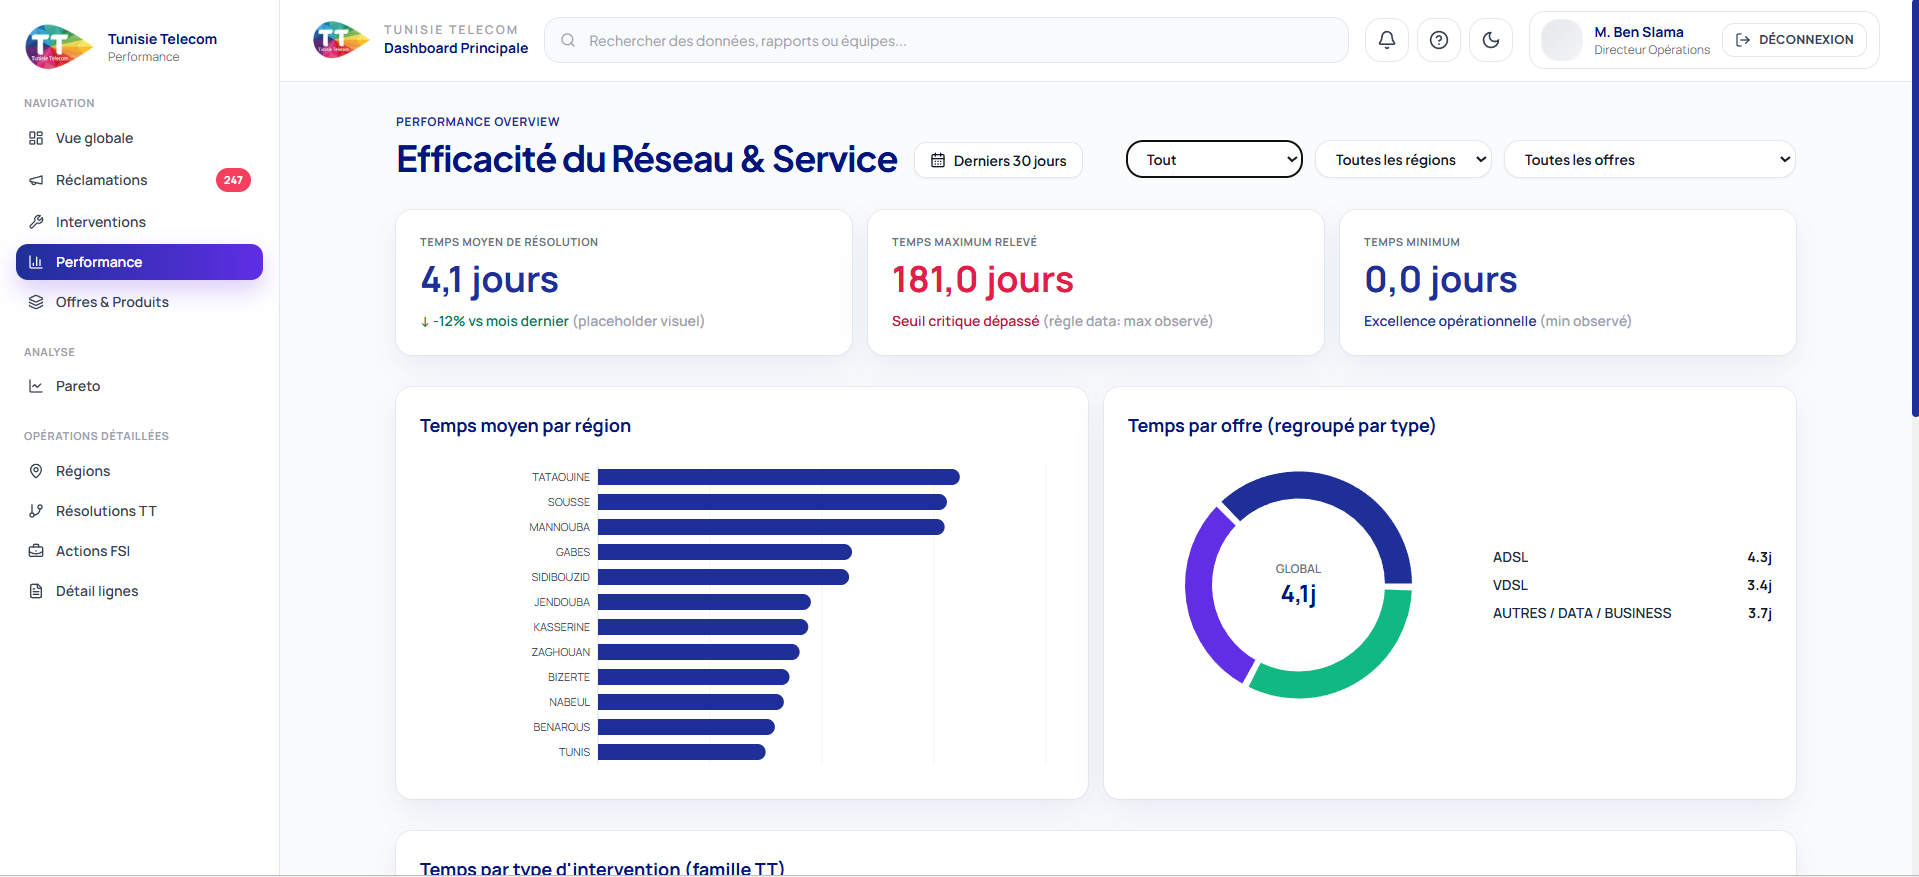
\includegraphics[width=0.85\textwidth]{imgs/04-dashboard-performance.png}
\caption{Vue Performance --- Analyse multidimensionnelle des délais de résolution}
\label{fig:vue-performance}
\end{figure}

\subsection{Vue Régions --- Analyse territoriale}

La Vue Régions offre une analyse territoriale complète avec 24 régions actives dans le jeu de données complet. Elle met en évidence que GAFSA concentre le volume le plus élevé (4\,560 tickets sur l'année), suivi de TUNIS (2\,043) et BÉJA (1\,647). Le croisement volume/délai est particulièrement révélateur~: GAFSA présente un délai moyen faible (31,3\,h) malgré son volume élevé, tandis que KASSERINE cumule un volume important (1\,502 tickets) et un délai moyen élevé (116,4\,h), signalant une région à forte priorité d'intervention pour les équipes de supervision.

\begin{figure}[H]
\centering
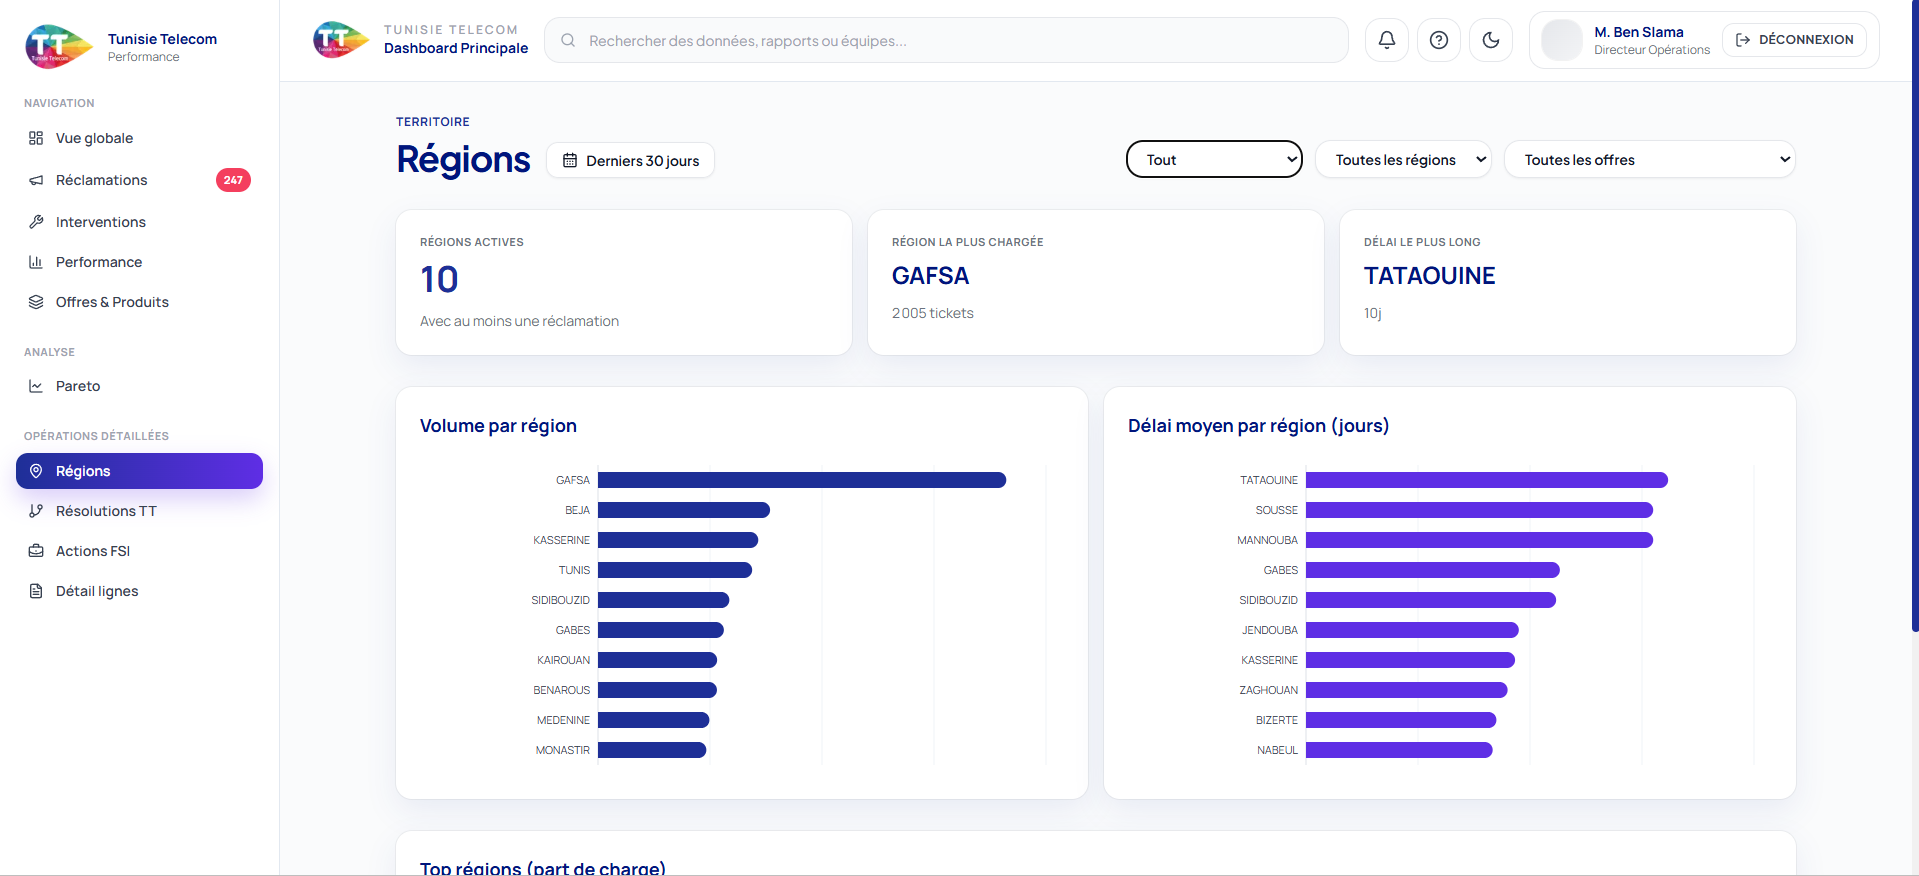
\includegraphics[width=0.85\textwidth]{imgs/07-dashboard-regions.png}
\caption{Vue Régions --- Analyse territoriale (volume et délai moyen par région)}
\label{fig:vue-regions}
\end{figure}

\subsection{Vue Résolutions TT --- Analyse qualité des actions}

La Vue Résolutions TT présente l'analyse détaillée des 12 codes de résolution distincts. Le graphique Pareto des codes de résolution confirme la concentration~: PC (2\,560 occ. --- 23,1\,\%), Aucun (2\,452 --- 22,1\,\%), IPMSAN (1\,801 --- 16,2\,\%) et Distribution (1\,067 --- 9,6\,\%) représentent ensemble 71,0\,\% du volume total sur le périmètre filtré. Le tableau de détail affiche pour chaque code~: volume absolu, fréquence relative (\%), cumul Pareto (\%) et conformité SLA (Excellent / Sous Objectif), permettant une lecture immédiate des priorités d'action.

\begin{figure}[H]
\centering
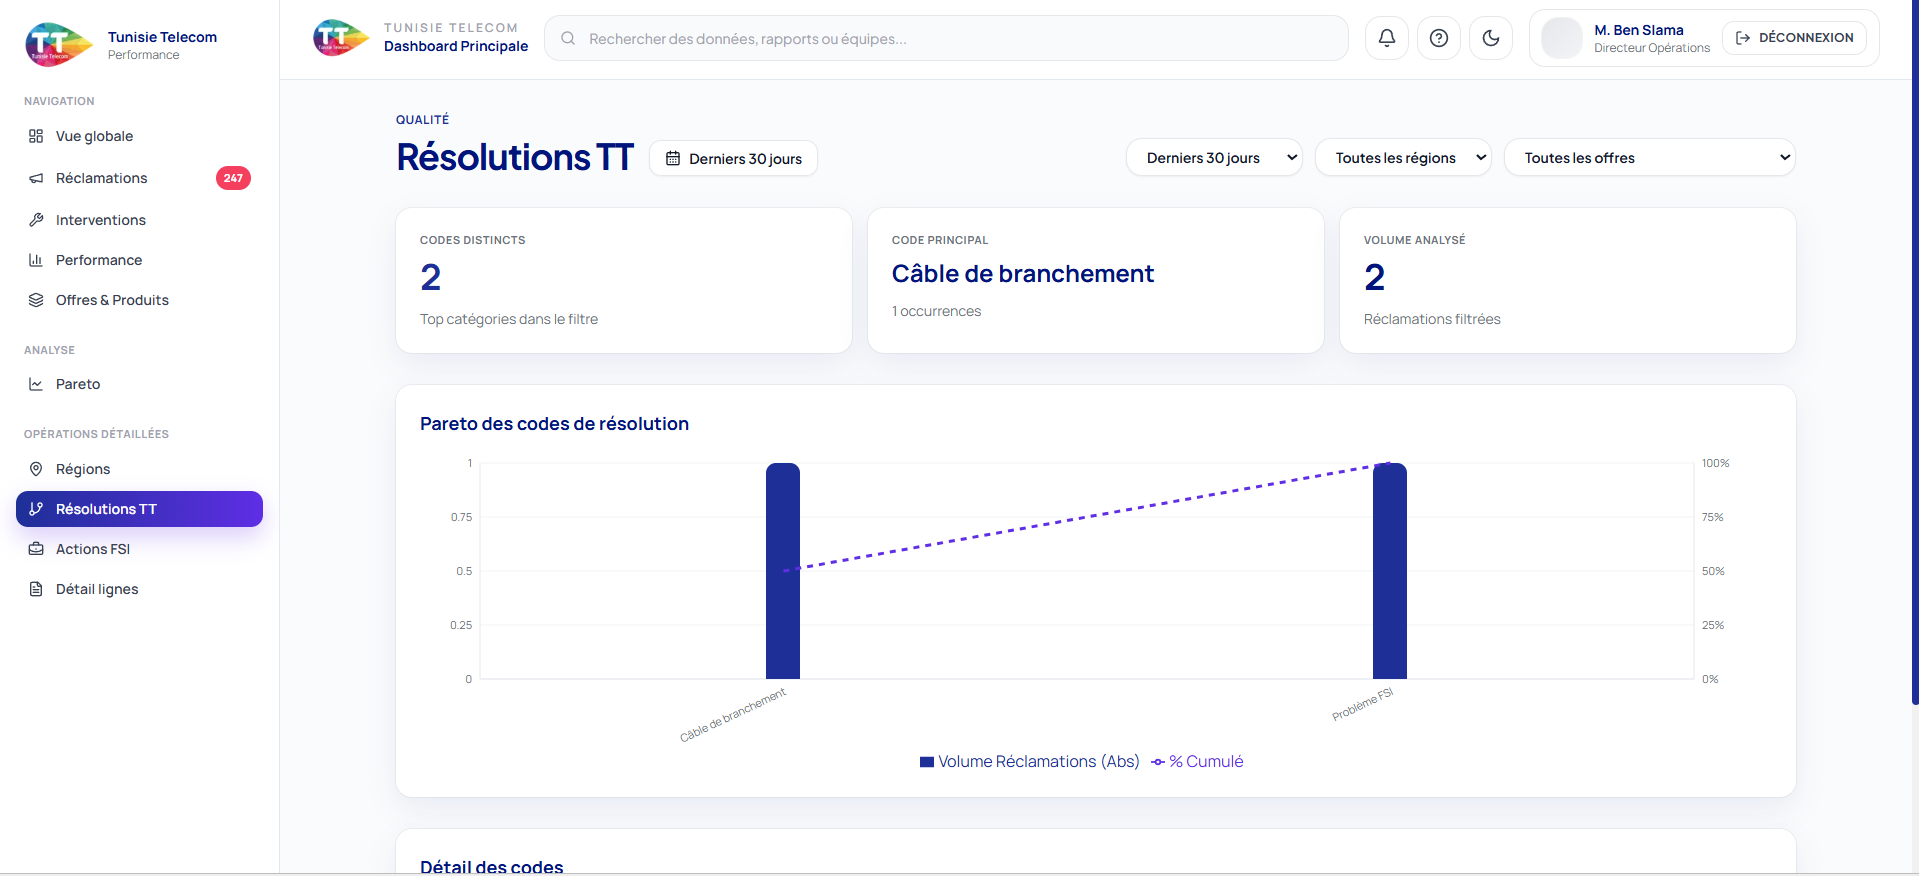
\includegraphics[width=0.85\textwidth]{imgs/08-dashboard-resolutions-tt.png}
\caption{Vue Résolutions TT --- Pareto des codes de résolution et tableau de détail}
\label{fig:vue-resolutions}
\end{figure}

\subsection{Vue Pareto --- Analyse Pareto intelligente}

La Vue Pareto constitue le module analytique central du dashboard. Elle intègre~:

\begin{itemize}[leftmargin=*, itemsep=4pt]
  \item Un \textbf{widget de génération de rapport Pareto intelligent} avec sélection de la portée (Mensuelle, Annuelle, Globale) et bouton « Générer le rapport ».
  \item Quatre \textbf{KPI cards de synthèse}~: Total Réclamations (11\,088), Délai Résolution (98,1\,h), Indice de Satisfaction (10/10 Neutre), Alertes Haute Priorité (2\,980 --- Critique).
  \item Un \textbf{graphique Pareto interactif} des codes de résolution avec deux modes d'affichage (Logique / Cumulatif).
  \item Un \textbf{classement des meilleures offres} par volume sur la période filtrée.
  \item Un \textbf{tableau de données détaillé} avec export CSV intégré.
\end{itemize}

\begin{figure}[H]
\centering
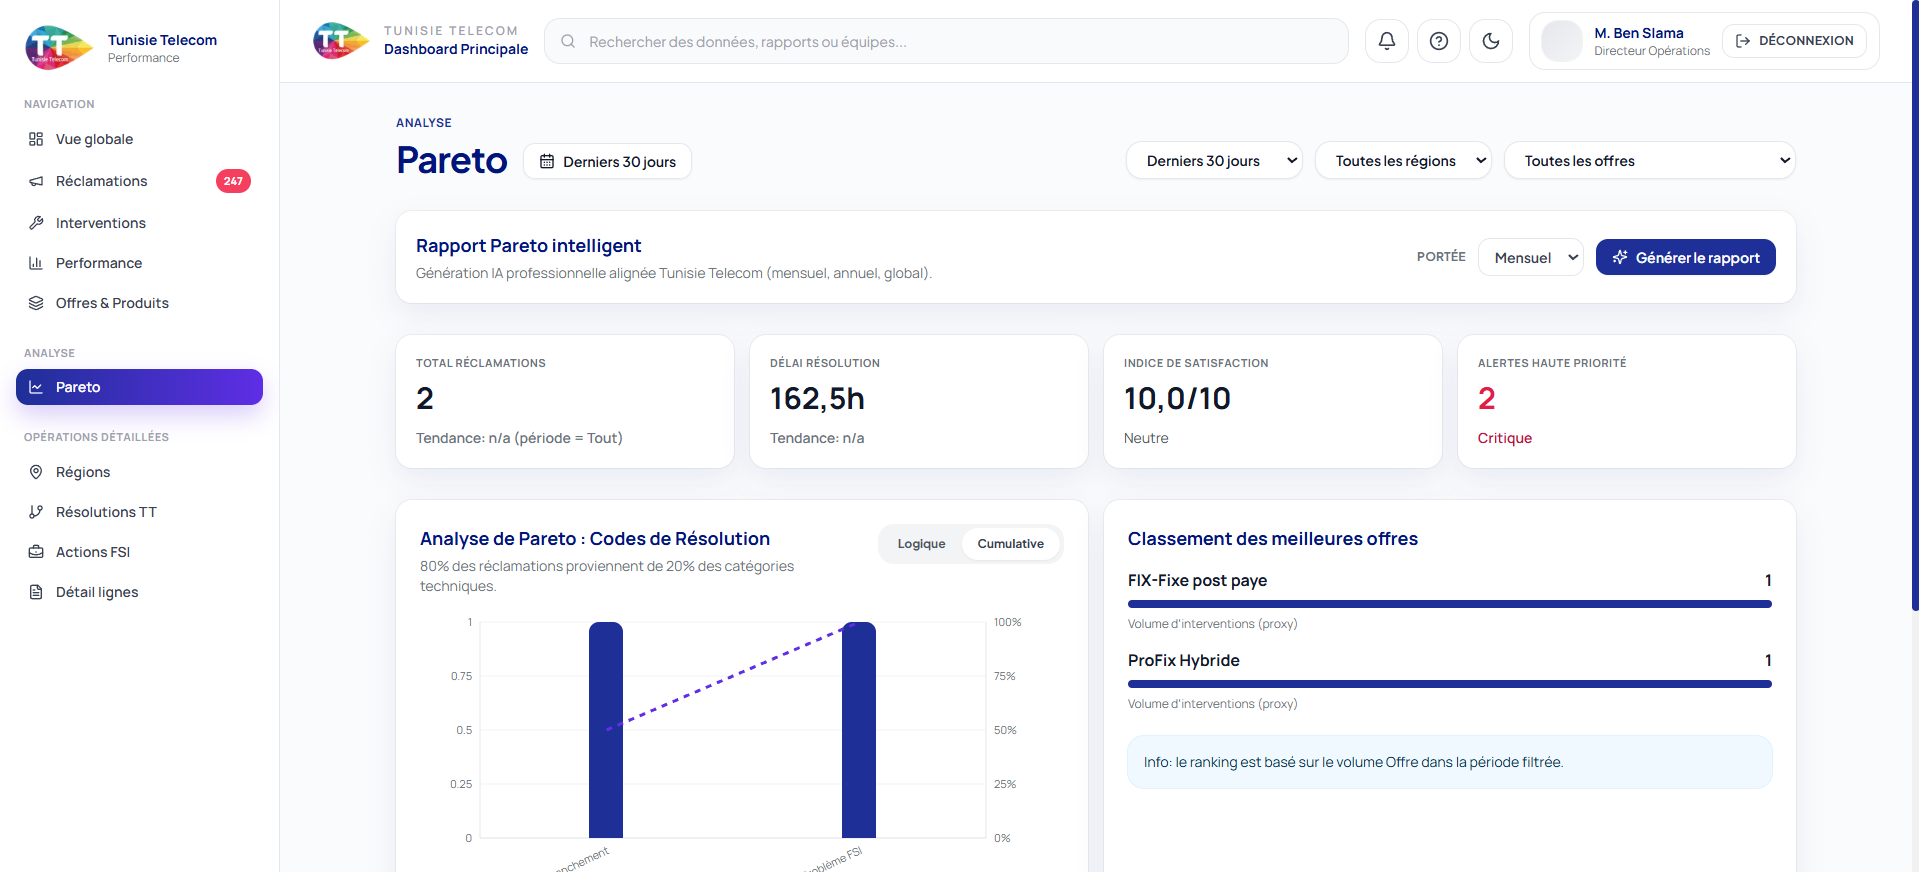
\includegraphics[width=0.85\textwidth]{imgs/06-dashboard-pareto.png}
\caption{Vue Pareto --- Analyse Pareto intelligente et module de génération de rapport IA}
\label{fig:vue-pareto}
\end{figure}

\section{Implémentation du Module Pareto Intelligent (IA)}

\subsection{Architecture du module IA}

Le module Pareto intelligent est implémenté sous la forme d'un \textit{Route Handler} Next.js (\texttt{/api/pareto/report}) qui, sur déclenchement par l'utilisateur, effectue les opérations suivantes~:

\begin{enumerate}[leftmargin=*, label=\arabic*., itemsep=4pt]
  \item Agrégation des données de réclamations selon le périmètre filtré (période, région, offre).
  \item Calcul du tableau Pareto (codes de résolution triés par volume décroissant, avec fréquence relative et cumul).
  \item Construction d'un prompt structuré en français, intégrant le contexte opérationnel Tunisie Telecom et les données agrégées.
  \item Appel à l'API Groq avec transmission du prompt et du modèle \texttt{llama-3.3-70b-versatile}.
  \item Restitution du rapport généré (texte structuré en langage naturel professionnel) dans l'interface.
\end{enumerate}

\subsection{Conception du prompt et calibrage du modèle}

La qualité du rapport généré repose en grande partie sur la conception du prompt soumis au modèle. Le prompt est structuré en trois sections distinctes~: (1) un \textbf{contexte opérationnel} précisant l'identité de l'opérateur (Tunisie Telecom), le rôle du destinataire (Directeur des Opérations) et la nature des données~; (2) les \textbf{données Pareto agrégées} (codes de résolution, volumes, fréquences, cumuls, conformité SLA)~; et (3) une \textbf{instruction de génération} précisant le format attendu (rapport professionnel en français, structuré en~: synthèse exécutive, analyse des causes prioritaires, recommandations d'actions correctives, conclusion).

\subsection{Extrait du code source}

\begin{lstlisting}[style=jsStyle, caption={Route Handler Next.js --- Module Pareto Intelligent (Groq / Llama 3.3 70B)}, label={lst:pareto-api}]
// src/app/api/pareto/report/route.ts
import { NextResponse } from "next/server";
import { loadDashboardIncidentsSafely } from "@/lib/dashboardData";
import { generateGroqText } from "@/lib/ai/groq";
import {
  buildParetoReportPayload,
  filtersForScope,
  normalizeRequestedFilters,
  paretoReportRequestSchema,
} from "@/lib/ai/paretoReport";
import { buildParetoSystemPrompt, buildParetoUserPrompt } from "@/lib/ai/paretoPrompt";

const DEFAULT_GROQ_MODEL = "llama-3.3-70b-versatile";

export async function POST(request: Request) {
  const parsedBody = paretoReportRequestSchema.safeParse(await request.json());
  if (!parsedBody.success) {
    return NextResponse.json({ error: "Parametres invalides" }, { status: 400 });
  }

  const dataSource = await loadDashboardIncidentsSafely();
  if (!dataSource.ok) {
    return NextResponse.json({ error: "Source de donnees indisponible" }, { status: 503 });
  }

  const baseFilters = normalizeRequestedFilters(parsedBody.data.filters);
  const appliedFilters = filtersForScope(baseFilters, parsedBody.data.scope);
  const payload = buildParetoReportPayload(dataSource.data, parsedBody.data.scope, appliedFilters);

  const reportText = await generateGroqText({
    apiKey: process.env.GROQ_API_KEY?.trim() ?? "",
    model: process.env.GROQ_MODEL?.trim() || DEFAULT_GROQ_MODEL,
    messages: [
      { role: "system", content: buildParetoSystemPrompt() },
      { role: "user", content: buildParetoUserPrompt(payload) },
    ],
    temperature: 0.15,
    maxTokens: 1500,
  });

  return NextResponse.json({ scope: payload.scope, reportText, metrics: payload });
}
\end{lstlisting}

\subsection{Exemple de rapport Pareto IA généré}

À titre d'illustration, voici un extrait représentatif d'un rapport généré par le module IA sur le périmètre Mensuel / Toutes régions / Toutes offres~:

\begin{tcolorbox}[insightbox, title=Extrait --- Rapport Pareto Intelligent (généré par Llama 3.3 70B / Groq)]
\textit{\small\textbf{Synthèse executive~:} L'analyse de la période considérée révèle un volume total de 11\,088 réclamations avec un taux de résolution de 99,9\,\%. Deux codes de résolution --- PC (23,1\,\%) et Aucun (22,1\,\%) --- concentrent à eux seuls 45,2\,\% du volume total, constituant les leviers d'action prioritaires pour l'amélioration de la performance.}

\medskip
\textit{\small\textbf{Recommandations~:} (1) Renforcer les équipes dédiées au code PC (Problème Câblage) dans les régions KASSERINE et SIDI BOUZID qui cumulent délai élevé et volume important. (2) Investiguer la cause racine des 22,1\,\% de tickets clôturés « Aucun » --- potentiellement des faux positifs du diagnostic FSI. (3) Prioriser la maintenance préventive du réseau de distribution dans les régions à fort cumul IPMSAN...}
\end{tcolorbox}

\section{Implémentation des Interfaces FSI et Agent TT}

\subsection{Espace fournisseur FSI}

L'Espace Fournisseur est accessible à \texttt{espace-fournisseur.vercel.app} et implémente le flux de gestion des réclamations décrit dans le chapitre de conception. La recherche par numéro DLigne vérifie en temps réel l'existence d'un ticket ouvert (contrôle de doublon). La création d'un ticket déclenche l'enregistrement dans le système et l'apparition immédiate du ticket dans l'Interface Agent TT. L'interface de tests techniques guide le FSI étape par étape dans l'exécution des tests de débit, synchronisation et connectivité requis avant et après l'intervention.

\subsection{Interface agent technicien TT}

L'Interface Agent TT est accessible à \texttt{espace-technicien.vercel.app}. Elle présente une liste filtrée des tickets à traiter (triés par urgence --- délai décroissant), avec indication visuelle des tickets dépassant 72\,h (badge rouge « Urgent »). L'écran de détail permet à l'agent de renseigner le code de résolution (menu déroulant parmi les 12 codes), la famille d'intervention, ses observations terrain, et de valider la clôture. La clôture déclenche automatiquement le calcul du KPI Délai de Résolution pour ce ticket et l'alimentation du dashboard de performance.

\chapconclusion{%
L'implémentation réalisée confirme la faisabilité technique du système SPPOI dans un cadre web moderne, avec une intégration effective des modules analytiques, métier et IA. La qualité de cette réalisation est ensuite évaluée dans le chapitre suivant à travers les tests, les validations fonctionnelles et l'analyse des résultats obtenus.%
}


% ═════════════════════════════════════════════════════════════════════════════
%  CHAPITRE 5
% ═════════════════════════════════════════════════════════════════════════════
\chapter{Tests, Validation et Résultats}

\chapintro{%
Ce dernier chapitre évalue le système réalisé à travers ses performances techniques, la qualité des résultats analytiques et les enseignements tirés de l'exploitation des données réelles. Il met également en évidence les limites observées afin de situer clairement le niveau de maturité de la solution proposée.%
}


\section{Présentation des Résultats Obtenus}

\subsection{Métriques de performance technique du système}

\begin{table}[H]
\centering
\caption{Métriques de performance technique du système SPPOI}
\begin{tabularx}{\textwidth}{L{5.5cm} C{3.5cm} C{3.5cm}}
\toprule
\rowcolor{ttlblue}
\textbf{\color{ttblue}Métrique} & \textbf{\color{ttblue}Valeur observée} & \textbf{\color{ttblue}Objectif cible} \\
\midrule
Temps de chargement Vue Globale   & $<$ 1,5\,s   & $<$ 3\,s \\
\rowcolor{ttlgray}
Temps de chargement Vue Pareto    & $<$ 2,0\,s   & $<$ 3\,s \\
Temps de génération rapport IA    & 3 à 8\,s     & $<$ 15\,s \\
\rowcolor{ttlgray}
Volume de données traité          & 22\,851 enreg. & $\geq$ 10\,000 \\
Disponibilité (Vercel)            & 99,99\,\%    & $\geq$ 99,5\,\% \\
\rowcolor{ttlgray}
Compatibilité navigateurs         & Chrome, Firefox, Edge, Safari & Navigateurs modernes \\
\bottomrule
\end{tabularx}
\label{tab:perf-tech}
\end{table}

\subsection{Principaux enseignements tirés de l'analyse des données réelles}

L'analyse systématique des 22\,851 tickets du jeu de données réel Fournisseur Anonyme 2025 a permis de dégager cinq enseignements opérationnels majeurs, directement restituables aux responsables de Tunisie Telecom via le dashboard~:

\begin{enumerate}[leftmargin=*, label=\textbf{\arabic*.}, itemsep=8pt]
  \item \textbf{Paradoxe performance/délais~:} Le taux de résolution de 99,93\,\% coexiste avec un délai moyen de 79,0\,h et une médiane de seulement 25,8\,h. Ce décalage traduit l'existence d'un sous-ensemble de tickets à durée de vie très longue (incidents infrastructurels complexes) qui tirent la moyenne vers le haut.

  \item \textbf{Concentration des causes (Pareto confirmé)~:} Six codes de résolution sur douze concentrent 81,6\,\% du volume des réclamations sur l'année. La loi de Pareto se vérifie avec une précision remarquable dans le contexte télécom tunisien.

  \item \textbf{Disparités régionales significatives~:} L'écart entre la région de Mannouba (délai moyen~: 180,8\,h) et les régions les plus performantes (GAFSA~: 31,3\,h) révèle des inégalités importantes dans la capacité de résolution régionale. KASSERINE cumule à la fois un volume élevé et un délai important (116,4\,h), en faisant la région à prioriser.

  \item \textbf{Dominance de l'ADSL et impact sur les délais~:} Avec 66,4\,\% du volume total (15\,163 tickets) et un délai moyen de 82,6\,h (contre 67,2\,h pour le VDSL), l'Offre de Gros ADSL Hybride est le segment le plus exposé aux incidents, orientant les priorités d'investissement vers la modernisation du réseau cuivre.

  \item \textbf{Saisonnalité thermique des incidents~:} Le pic de juillet~2025 (2\,129 tickets --- volume mensuel maximum) et le creux de février~2025 (1\,708 tickets) confirment une saisonnalité liée aux conditions climatiques, ouvrant la voie à des modèles prédictifs de planification des ressources.
\end{enumerate}

\subsection{Retour d'expérience et limites identifiées}

Malgré les résultats satisfaisants obtenus, plusieurs limitations du système actuel méritent d'être signalées de manière transparente~:

\begin{itemize}[leftmargin=*, itemsep=6pt]
  \item \textbf{Source de données statique~:} Le système actuel s'appuie sur un fichier Excel fourni par le Fournisseur Anonyme, sans connexion directe aux systèmes HPSM et Extranet de Tunisie Telecom. Cette architecture implique une mise à jour manuelle périodique des données.

  \item \textbf{Périmètre fournisseur unique~:} Les données disponibles ne couvrent qu'un fournisseur anonyme. L'extension à l'ensemble des FSI partenaires de Tunisie Telecom nécessiterait une phase d'intégration supplémentaire.

  \item \textbf{Authentification basique~:} La version actuelle implémente une authentification par rôle simplifiée, sans intégration avec le système d'authentification centralisé de Tunisie Telecom.

  \item \textbf{Module IA dépendant d'un service cloud tiers~:} La génération des rapports Pareto intelligents repose sur l'API Groq, service externe. Une indisponibilité de ce service impacterait le module IA sans affecter le reste du dashboard.
\end{itemize}

\chapconclusion{%
Les tests et résultats obtenus montrent que le système répond de manière satisfaisante aux objectifs initiaux de pilotage, d'analyse et d'aide à la décision. Malgré certaines limites liées au périmètre de données et à l'intégration SI, le SPPOI constitue une base opérationnelle crédible pour une généralisation et un enrichissement futurs.%
}

% ─────────────────────────────────────────────────────────────────────────────
%  CONCLUSION GÉNÉRALE ET PERSPECTIVES
% ─────────────────────────────────────────────────────────────────────────────
\chapter*{Conclusion Générale et Perspectives}
\addcontentsline{toc}{chapter}{Conclusion Générale et Perspectives}
\thispagestyle{fancy}

Ce projet a permis de concevoir et de mettre en œuvre un système cohérent de pilotage de la performance des interventions, adapté aux besoins opérationnels observés chez Tunisie Telecom. À partir d'un besoin réel de visibilité, de consolidation et d'aide à la décision, la solution développée structure l'information disponible, facilite l'interprétation des indicateurs et renforce la capacité de réaction face aux dérives de performance.

Les résultats obtenus confirment l'intérêt de l'approche retenue. Le dashboard principal apporte une lecture synthétique et détaillée de la situation opérationnelle, les interfaces métier améliorent la continuité du traitement entre acteurs, et le module Pareto intelligent enrichit l'analyse par une restitution rédigée et contextualisée des priorités d'action. L'ensemble constitue une base crédible pour un pilotage plus lisible, plus rapide et plus orienté résultat.

Plusieurs perspectives d'évolution peuvent être envisagées. Une première consiste à automatiser complètement l'alimentation des données par connexion directe aux systèmes de production. Une deuxième porte sur l'extension du périmètre à l'ensemble des fournisseurs partenaires et à d'autres services télécom. Enfin, l'ajout de modèles prédictifs complémentaires permettrait d'anticiper les pics d'incidents, d'optimiser la planification des ressources et de renforcer la maintenance proactive.

Ainsi, le SPPOI constitue non seulement une réponse concrète au besoin exprimé dans le cadre de ce projet, mais également une base évolutive pour une transformation plus large du pilotage opérationnel des dérangements.


% ═════════════════════════════════════════════════════════════════════════════
%  BIBLIOGRAPHIE
% ═════════════════════════════════════════════════════════════════════════════
\begin{thebibliography}{99}
\addcontentsline{toc}{chapter}{Bibliographie}

\bibitem{kaplan1996}
R.~S. Kaplan et D.~P. Norton, \textit{The Balanced Scorecard: Translating Strategy into Action}, Harvard Business School Press, Boston, 1996.

\bibitem{imai1986}
M.~Imai, \textit{Kaizen: The Key to Japan's Competitive Success}, McGraw-Hill, New York, 1986.

\bibitem{deming1982}
W.~E. Deming, \textit{Out of the Crisis}, MIT Press, Cambridge, 1982.

\bibitem{itil2019}
AXELOS, \textit{ITIL\textsuperscript{\textregistered} Foundation: ITIL 4 Edition}, The Stationery Office (TSO), Norwich, 2019.

\bibitem{iso20000}
ISO/IEC 20000-1:2018, \textit{Information Technology --- Service Management --- Part 1: Service Management System Requirements}, International Organization for Standardization, Geneva, 2018.

\bibitem{rockart1979}
J.~F. Rockart, ``Chief Executives Define Their Own Data Needs,'' \textit{Harvard Business Review}, vol.~57, no.~2, pp.~81--93, 1979.

\bibitem{nextjs2025}
Vercel Inc., \textit{Next.js Documentation --- App Router}, Documentation officielle, \url{https://nextjs.org/docs}, consulté en 2025.

\bibitem{meta2024}
Meta AI Research, \textit{Llama 3: Open Foundation and Fine-Tuned Chat Models}, Meta AI Technical Report, 2024.

\bibitem{groq2025}
Groq Inc., \textit{Groq API Documentation --- Language Processing Units (LPU) Inference Engine}, \url{https://console.groq.com/docs}, consulté en 2025.

\bibitem{recharts2025}
Recharts Team, \textit{Recharts --- Redefined chart library built with React and D3}, \url{https://recharts.org}, consulté en 2025.

\bibitem{tailwind2025}
Tailwind CSS Team, \textit{Tailwind CSS --- A Utility-First CSS Framework}, \url{https://tailwindcss.com/docs}, consulté en 2025.

\bibitem{sheetjs2025}
SheetJS Community, \textit{SheetJS CE --- Spreadsheet Data Toolkit}, \url{https://sheetjs.com/docs}, consulté en 2025.

\bibitem{tt2024}
Tunisie Telecom, \textit{Rapport Annuel 2024}, Direction de la Communication, Tunis, 2024.

\bibitem{ins2024}
Institut National de la Statistique (INS) Tunisie, \textit{Indicateurs du secteur des télécommunications en Tunisie}, INS, Tunis, 2024.

\bibitem{pbi2024}
Microsoft Corporation, \textit{Power BI Documentation --- Business Intelligence and Analytics}, \url{https://docs.microsoft.com/power-bi}, consulté en 2025.

\end{thebibliography}


\end{document}
